\documentclass[a4paper,11pt,twoside]{report}

%\usepackage{config/UmUThesis}           % Standard English
\usepackage[noindent]{config/UmUThesis}  % Non indented English
%\usepackage[se]{config/UmUThesis}       % Swedish

\usepackage[applemac]{inputenc}
\usepackage{courier}              % Nicer fonts are used. (not necessary)
\usepackage{pslatex}              % Also nicer fonts. (not necessary)
\usepackage{lmodern}              % Optional fonts. (not necessary)
\usepackage{url}
\usepackage[T1]{fontenc}

\usepackage{subcaption}
\usepackage{csquotes}

\usepackage{adjustbox}
\usepackage{graphicx}

\usepackage{blindtext}
\usepackage{amssymb}
\usepackage{pifont}
\usepackage[inline]{enumitem}

\newcommand{\ignore}[1]{}

	\title{User onboarding for mobile applications: A design guideline}
	\author{Simon Johansson}
	\supervisor{Staffan Grundberg}
	\supervisore{}
	\examiner{Ulrik S\"{o}derstr\"{o}m}
	\semester{Spring 2017}
	\course{Master Thesis, 30 hp}
	\education{M.Sc. Interaction Technology and Design, 300 hp}

\graphicspath{{resources/images/}}
\pagestyle{empty}

\begin{document}
\maketitle

%%-----------------------------------------------------------------------------------------------------------------
%%----------ACKNOWLEDGEMENTS---------------------------------------------------------------------
%%-----------------------------------------------------------------------------------------------------------------

\begin{center}
\section*{Acknowledgements}
Thanks mum and dad \ding{164}
\end{center}

\clearpage

%%-----------------------------------------------------------------------------------------------------------------
%%------------ABSTRACT-------------------------------------------------------------------------------------
%%-----------------------------------------------------------------------------------------------------------------

\begin{center}
\section*{Abstract}
Abstract, abstract, abstract...
% WRITE IN PRESENT TENSE!

%%% 1. Explanation of the title of your thesis
% The first function of the abstract is to further explain the title of your thesis. This allows readers of tour thesis to better determine if your thesis is interesting enough for them to read. A well-written abstract can encourage more people to consider your thesis important and, thus, to intend to read it.

%%% 2. Short version of your thesis
% The abstract serves as a short version for readers who don?t have the time to read the complete thesis. Often, managers and scientists read only the abstract and not the entire piece.

%%% 3. Overview of your thesis
% The abstract?s function is to serve as an overview of what readers can expect. This makes it easier for the reader to understand and to place in context the material in the thesis. A well-written abstract ensures that difficult material in your thesis is better understood.

% - What is the problem? Indicate the objective, problem statement and research questions of your thesis. If you have used hypotheses in your thesis, indicate them here.
% - What has been done? Briefly explain the method and approach of your research
% - What has been discovered? Provide a summary of the most important results and your conclusion
% - What do your findings mean? Summarize the key points from the discussion and present your recommendations

%% Understand your abstract without going through the rest of your thesis.
%% Include references when you use a source. You often do not use any references because you mainly write about your own findings and research

%% --------------------------- CHECKLIST -------------------------------------
% - Maximum of A4 sheet of paper
% - Placed after the preface and before the table of contents
% - Written in present tense
% - The objective is specified
% - The problem statement is given
% - The research questions or hypotheses are included
% - The methodology and approach of your research are briefly explained
% - A summary of the most important results are given
% - The conclusion is given (the answer to your research question / problem statement).
% - The results have been discussed and explained (discussion).
% - Suggestions for follow-up research are presented
% - Any recommendations are concisely discussed
% - The abstract clarifies what the thesis is about

\end{center}

\setcounter{page}{1}

%%-----------------------------------------------------------------------------------------------------------------
%%----------TABLE OF CONTENTS----------------------------------------------------------------------
%%-----------------------------------------------------------------------------------------------------------------

\tableofcontents

%% The chapter 'Introduction' will introduce the reader to field of research, mention some earlier and related work, introduce the company Doberman and the product which we will test
\chapter{Introduction}
\label{chap:introduction}

%% Establish the territory [the situation]
You only have one chance to make a good first impression. The amount of apps smartphone users download on a monthly basis has been steadily decreasing since the launch of the smartphone in 2004 [1], and the founder of Mobilewalla suggest that users eventually uninstall 80-90\% of all downloaded apps \footnote{\url{http://usatoday30.usatoday.com/MONEY/usaedition/2012-01-31-App-Love-is-Fleeting\_ST\_U.htm}}, and 22\% of mobile users use an app only one before uninstall \footnote{\url{http://www.slideshare.net/vaibhavkubadia75/mobile-web-vs-mobile-apps-27540693?from_search=1}}. The reason a user might uninstall an app and what makes an app "bad" has been previously researched \cite{Lin2012} \cite{Shklovski} \cite{Song2014}. The reasons found for uninstalling vary with privacy/security concerns, didn't meet users expectations, didn't use the app often etc. Some of the reasons for uninstalling might be hard to account for, but designers and developers can at least help the user understand what the apps' value proposition is, and if the value proposition meets the users' need and expectation, help the user transition from a novice to a proficient user.

The term onboarding is a quite recent term \cite{Dai2007}. The term onboarding stems from a business, management and human-resource context, and it describes a process to introduce and help a new employee become an effective member of their new organization by teaching them the knowledge, skills and behaviors required to succeed \cite{Bauer2011}. Some study has identified that onboarding in a business context has a lot in common with user onboarding, since it contains a lot of the same aspects of bringing them up to speed and making them comfortable in their new environment. There are a lot of different opinions and thoughts about what a onboarding process entail, and when a employee or user has been successfully "onboarded".

Successfully onboarding a user will increase user retention (ref), and

There hasn't been a lot of academic research in the field of user onboarding, even though there's a lot of research regarding employee and manager onboarding (ref) (ref) (ref). The most notable contributions to the research field of user onboarding is by Oechsner, where she presents general guidelines for onboarding a user to a digital platform. Her guidelines are supported by psychology and IxD research, but fail to include the body of work of employee onboarding. Also, her guidelines are meant to be general and may not alone aid the the entire process of all platforms. This

% Define onboarding in a business context
% Talk about the problems inherited, and explain it in an user onboarding context.

, as defined by  is a process designed by developers and designers to help the user familiarize themselves with the application, its value proposition and. The onboarding process helps the user grow from a noob to a re

% WRITE IN PRESENT TENSE
% C.A.R.S model

% Describe the topic of your thesis
% Formulate the problem statement
% Write an overview of your thesis

% Although the introduction is at the beginning of your thesis, this placement does not mean that you must finish the introduction before you can start the rest of your research. The further you get in your research, the easier it will be to write a good introduction that is to the point. Thus, it is no disaster if you ca not write a perfect introduction right away.

%% 	PURPOSE OF THE INTRODUCTION
% - Introduce the topic. What is the purpose of the study and what is the topic?
% - Gain the readers interest. Make sure that you get the readers attention by using clear examples from recent news items or everyday life.
% - Demonstrate the relevance of the study. Convince the reader of the scientific and practical relevance.

%%%%%% PARTS OF THE INTRODUCTION
%%% - Motivation
% What is the motive for your research? This can be a recent news item or something that has always interested you.

%%% - Scope
% Based on the motivation or problem indication, you describe the topic of your thesis. Make sure that you directly define the topic of your research.

%%% - Theoretical and practical relevance of the research
% Using arguments, state the scientific relevance of your research.
% Highlight here the discussion chapters of studies that you are going to use for your own research.
% Explain the practical use of your research.
% When you are writing a thesis for a company, you will find that the scientific relevance is much more difficult to demonstrate. On the other hand, it should be easier to show the practical benefit. Think of, for example, the practical applications for the entire industry.

%%% - Current scientific situation
% Specify the most important scientific articles that relate to your topic and you briefly explain them.
% Show that many studies have been conducted around the topic, and that you won't get stuck due to finding too little information on your topic.

%%% - Objective of the study and the problem statement
% Describe the objective of your study and the problem statement that you have formulated.

%%% - Brief description of the research design
% Provide a brief summary of your research design. How, where, when and with whom are you going to conduct your research?

%%% - Thesis outline
% Briefly describe how your thesis is constructed. Summarize each chapter briefly in one paragraph at the most, but preferably in one sentence.
% Make sure your thesis outline is not repetitively phrased because it does not vary its word choice.

% Do not repeat yourself and only write down what is important to introduce your topic and research.

%% --------------------------- CHECKLIST -------------------------------------
% - Introduction of the research is written with a stimulating topic.
% - The topic is limited
% - The scientific relevance is demonstrated (not always applicable)
% - The practical relevance is demonstrated
% - The most important scientific articles about the topic are summarized
% - The objective is formulated
% - The problem statement is formulated
% - The conceptual framework is determined
% - The research question or hypotheses are formulated
% - The research design is described briefly
% - The thesis overview is added

\section{}

\section{Objective}

\section{Limitations}

\section{Goals}

\begin{itemize}
	\item
	\item
	\item
\end{itemize}

\section{Terminology}

\begin{tabular}{ | p{5.5cm} | p{6.5cm} |  }
	\hline
     	\multicolumn{2}{|c|}{Common terms and their explanation} \\
     	\hline
	     Field of View (FOV) & Explanation goes here. \\
    	\hline
     	Head-Mounted Display (HMD) & Explanation goes here. \\
    	\hline
     	Virtual Reality (VR) & Explanation goes here. \\
    	\hline
	Virtual Environment (VE) & Explanation goes here. \\
     	\hline
    	Omidirectional video (ODV) & Explanation goes here. \\
    	\hline
     	360� video & Explanation goes here. \\
     	\hline
     	3D video & Explanation goes here. \\
     	\hline
     	Hypervideo & Explanation goes here. \\
	\hline
\end{tabular}


%% The background will include background about the research field and my study
\chapter{Background}
\label{chap:background}


%% The Methodology will present how the study will be conducted
\chapter{Methodology}
\label{chap:methodology}
% In the study or research design, you explain where, when, how and with whom you are going to do the research.
% The question of 'how' will determine your research method. Are you gong to conduct research using a survey or perhaps with an experiment?

\section{Literature study}
A literature study is conducted to get an understanding of the research field of onboarding. The material for this study is mostly retrieved through the Google Scholar search engine and the "Digitala Vetenskapliga Arkivet" (DiVA) portal. This material is complemented with eventual articles, blogs and videos. The conclusion of the literature study is presented in the chapter \ref{chap:theoretical_framework}.

\section{Interviews}
%
\section{Best Practice Evaluation}
%
\section{Application review}
%
\section{User Testing}
%
\section{Personas}
%
\section{Prototypes}


%% The theoretical framework will present material for us to understand the resulting framework, which is also presented in this chapter, which also contain the results from the best practice analysis.
\chapter{Theoretical Framework}
\label{chap:theoretical_framework}
The theoretical framework consists of two main sections: \ref{sec:theoretical_background} and \ref{sec:best_practice_evaluation}

% Understanding experience
% http://repository.cmu.edu/cgi/viewcontent.cgi?article=1045&context=hcii

\section{Theoretical Background}
\label{sec:theoretical_background}
% User problems -> Mobile -> Value proposition
To better understand how to provide a good onboarding experience for the mobile app user we have to understand the problems associated with UX-design, both in general and problem mobile devices. We then structure the Theoretical Background with the subsections \textit{acquisition}, \textit{accommodation}, \textit{assimilation} and \textit{acceleration}. These concepts stems from business management context, but to explain them in a user-experience we draw inspiration from cognitive and behavioral psychology. Cognitive psychology is a branch of psychology which study higher mental processes of the human mind such as attention, language use, memory, perception, problem solving, and thinking \footnote{\url{http://www.apa.org/research/action/glossary.aspx?tab=3}}. Behavioral psychology and its research field is focused on the environmental determinants of learning and behavior. With the combined resources of these fields of research we define motivations of users to use an applications.

\subsection{Experience}
"Understanding experience is a critical issue for a variety of professions, especially design" \cite{Forlizzi2004}. Forlizzi and Battarbee has identified three different types of experiences; \textit{experience}, \textit{an experience} and \textit{co-experience}.

They claim that an \textit{experience} is a "constant stream of 'self-talk' that happens while we are conscious". This type of experience is, at any given time, how we assess the people, products and environment around us relative to our goals. This type of experience is usually ill-defined for the person, and usually does not have a start or end.

\textit{An experience}, on the other hand, can be articulated by the person who have experienced it. The experience is perceived through the interactions and emotions of the person, and the experience may illicit behavioral and emotional changes. As an experience has been experienced, the person has a sense of completion of the experience and it is stored and categorized in ones mind.

\textit{Co-experience} is about the joined experienced in a social context, and is created or shared together with others. Co-experience is further explained in Section \ref{sec:assimilation}.

\subsection{Acquisition}
% Acqusition Få tag i och förstå sina användare. Hur gör man detta? Man definierar och designar för sin målgrupp, och förstår deras motivation och ge dem vad de behöver. Det finns metoder för detta så som att skapa Personas. Det finns även ett problem så som marknadsföring och app discoverability, men vi ska inte täcka det i denna rapport.
Acquisition is the act of identifying, recruiting, selecting and getting people to join \cite{Bradt2009}. In this section we discuss important concepts such as \textit{Needs}, \textit{Motivation} and two models that describe human behavior; the \textit{Technology Acceptance Model} and \textit{Foggs' Behavioral Model}. Last we discuss the \textit{innovation diffusion theory}.

\subsubsection{Needs}
% Identify the motivation of the user base, explain what motivation is.
To be able to understand how to provide a good user experience, we have to understand the needs of the user, and what value is important to the user to fulfill their need. Maslow’s theory of motivation \cite{Maslow1943} state that humans are motivated by a hierarchy of needs; The 'physiological', the safety, the love, the esteem need and finally the need of self-actualization. Physiological needs are the classic instances of hunger, sex and thirst. Serving one of needs may act as a channel for other needs; someone might be eating because they seek comport rather than for vitamins or nutrients. He explains that when one hierarchy of need has been satisfied the human try to satisfy the next need in the hierarchy, and that the subsequent need has to be fulfilled to be able to care for any of the other needs; "A person who is lacking food, safety, love, and esteem would most probably hunger for food more strongly than for anything else.". The need for safety is the act of seeking a stability in the world where we are away from dangers. If both the physiological and the safety needs are met, then the need for love and belongingness is at the center of concern. The person is now concerned with having friends, a partner and/or children, and will take great strides to do so. When the esteem needs emerge after we have satisfied the physiological, safety and love needs, we strive for a high evaluation of ourselves, for self-respect, or self-esteem, and for the esteem of others. We want to be respected and valued by others, and this need may strive people to engage in a profession or hobby to gain recognition. Maslow states that this need can be divided into two sets. The first is the desire of self-respect, independence and freedom. Secondly we have the desire for respect from others. Finally, when all precedent needs have been satisfied we reach the need for self-actualization, which refers to the need of self-fulfillment. "What a man \textit{can} be, he \textit{must} be"

% Read Hazzenzahl 2010

\subsubsection{Motivation}

Motivation is what drives human to accomplish things, keeps them interested and committed \ignore{\cite{Ryan and Deci, 2000}}.

It is not the need --- previously discussed in Section \ref{subsubsec:needs} --- that motivate people, but the goal to satisfy the need \cite{Maslow1943}. Also, most motivated actions are not to satisfy just one need, but to satisfy multiple needs. A man or woman might partially eat to satisfy hunger and partially feel comfort.

At the level of self-determination, we distinguish between different types of motivation; \textit{intrinsic} and \textit{extrinsic} motivation \cite{Ryan2000a}. These differ in the reason or goal that prompts the execution of some action. Intrinsic motivation specifically refers to the act of doing something due to it being interesting or enjoyable, and extrinsic motivation refers to the act of doing something because it leads to a favorable outcome. The word \textit{Intrinsic} is defined as "belonging to a thing by its very nature"\footnote{\url{http://www.dictionary.com/browse/intrinsic}}, and intrinsic motivation is thought to be a fundamental aspect of the human creature \cite{White1959}. Since we were born, we have had a curiosity of the world with no external incentives to learn and explore it \cite{Ryan2000a}. Extrinsic motivation is the underlying reason an activity is performed to attain some outcome. The final outcome is the facilitator of the activity, and not the activity itself \cite{Ryan2000a}. This is also the main problem with extrinsic motivation; when the external factors disappear so does the motivation\ignore{\cite{Hassenzahl2010}}. It is believed from operant theory that all behaviors are motivated by rewards\ignore{\cite{Skinner1953}}, therefore intrinsically motivated people perform a task because the task itself is rewarding to them, while extrinsically motivated people only perform it to achieve the external reward. Research suggest that higher levels of intrinsic motivation typically lead to a higher willingness to spend more time on a task \cite{Deci1975}. Intrinsic motivation is regarded as the better of the two when designing user experiences, but may be harder for the designer to create.

To improve the users intrinsic motivation, the user interface designer can relate the content and objectives of the application to the needs and interests of the learner \ignore{\cite{Keller1983}}. This can be done by using familiar metaphors and analogies \ignore{\cite{Curtis1984}}. Instructions provided to the user that use a personal style (e.g personal pronouns, names of specific people) rather than formal style may stimulate the user to learn. Also, providing immediate, positive and informative feedback in a context may improve intrinsic motivation, but not necessarily increase or decrease performance \ignore{\cite{(Bates, 1979; Condry, 1977; Deci, 1975, 1971; Keller, 1983)}}. Humor, on the the other hand, has been found to not improve motivation since it can distract the user and interfere with comprehension \ignore{\cite{Markiewicz, 1974; Sternthal & Craig, 1973}}.

Motivation will not alone prompt a user to perform a target behavior. The following sections will discuss two models developed for understanding user informational system adoptance and a behavioral model for persuasive design.

\subsubsection{Technology Acceptance Model}
While there are other theoretical models developed to explain user acceptance and usage behaviour of information technologies, the Technology Acceptance Model (TAM) \cite{Davis1989} \cite{Davis1989a} is the most widely accepted model and has been validated numerous times, e.g. \cite{Hu1999} \cite{Chau1996} \cite{Mathieson1991}. TAM explain the behavioral intention to use an technology with two major beliefs; \textit{perceived ease of use} and \textit{perceived usefulness}. Perceived ease of use is how much a person believes that the use of some technology will be free of effort. This is believed to be a process of expectancy, since the perceived ease of use is defined in terms of expected effort the user is able to report whether or not their expectancy is correct. Perceived usefulness is how much a person believes that using a technology will enhance their productivity. These two beliefs correlate with each other, as perceived usefulness is an outcome of the users expectancy. A positive perceived ease of use will positively influence perceived usefulness, as when the technology is easier to use, the more useful it can be. Davis \cite{Davis1989} has found that perceived ease of use has a direct effect on intention, and in an indirect effect on intention via perceived usefulness, and that it is an initial hurdle for users to overcome for acceptance, adoption and usage of a system \cite{Davis1989a}. Figure \ref{fig:TAM} represent the theoretical model.

\begin{figure}[h]
  \centering
    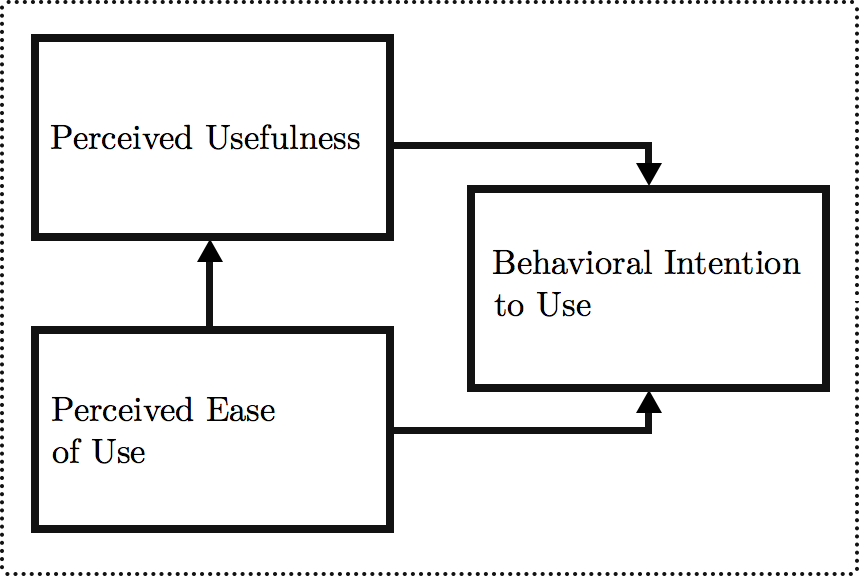
\includegraphics[width=0.6\textwidth]{TAM}
  \caption{Theoretical model of Technology Acceptance Model (modified from \cite{Davis1989}).}
  \label{fig:TAM}
\end{figure}

This model implicitly indicate that external variables influence perceived ease of use and perceived usefulness. There has been several studies which has defined some of these external variables and extended the model with constructs such as intrinsic motivation, control, emotion \cite{Venkatesh2000}, flow theory \cite{Koufaris2002} and trust \cite{Gefen2003}.

To design an interface to increase perceived ease of use there are a number of ways we can do this. Tractinsky et al. has found a strong correlation between aesthetics and perceived usability, which remain intact from the users initial use to continued use \cite{Tractinsky2000}.

\ignore{
System designers typically attempt to build systems that are easy to use while providing the functionality that the users need to accomplish their tasks. While user interface design is the typical focal point to enhance user acceptance, this research shows that there are multiple factors not directly related to the user system interaction that are perhaps more important (e.g., computer self-efficacy). While a large amount of time during system design and development is typically spent on the user interface, this research suggests that practitioners should spend more time creating a favorable impact on system-independent factors, which have clearly been shown to be more important than user perceptions that relate to the user-system interaction in determining perceived ease of use of a specific system. This is particularly important since at all stages of user experience with a system, general, system-independent constructs play a stronger role than constructs that are a result of the user-system interaction.

Similarly, research should focus on designing managerial interventions that will provide facilitating conditions that favor the creation of positive perceptions about the ease of use of a specific system via perceptions of external control. Researchers and practitioners should attempt to better leverage the individual difference variable of computer playfulness and system-specific perceived enjoyment during the design and development phases of system building, and attempt to incorporate it into end-user training situations. In general, practitioners should design interventions directed at the various determinants of perceived ease of use that go beyond traditional training methods, which typically aim to impart only conceptual and procedural knowledge about a specific system. Organizations should consider putting in place general computer training programs that target increasing computer awareness, enhancing computer self-efficacy, and reducing computer anxiety among employees. Such training programs combined with appropriate facilitating conditions should pave the path for acceptance and usage of new systems. In fact, organizations will benefit particularly from system-specific training interventions that enhance user perceptions about the specific system and their general beliefs about new information technologies (see Compeau 1992).
One of the areas that has not been exploited in practice is the potential for intrinsic motivation to enhance user acceptance and usage. Much prior research (Davisetal.1992;Malone1981a,1981b;Websterand Martocchio 1992; Venkatesh and Speier 1999) has found intrinsic motivation to be an important factor influencing user acceptance and learning. This research has further refined our understanding in this regard by suggesting that general computer playfulness and perceived enjoyment are determinants of perceived ease of use. One example is “fun icons” like the ones introduced in MS-Office 97. A similar example is the use of “warm and fuzzy” screen savers (e.g., flashing cartoons on the screen, some action related to your favorite basketball team, etc.) as a way to cause perceived ease of use of specific systems (used by the individual) to be more favorable. Recent work in IS (Venkatesh 1999) and organizational behavior}

\subsubsection{Foggs' behavior model}
Fogg has developed a model to understand human behavior, called Foggs Behavior Model (FBM) \cite{Fogg2009}. The model states that for a target behavior to happen, the person must have sufficient \textit{motivation}, \textit{ability} and some effective event to \textit{trigger} the behavior. The model is visualized in Figure \ref{fig:FBM}.

\begin{figure}[h]
  \centering
    \includegraphics[width=0.8\textwidth]{FBM}
  \caption{Foggs Behavioral Model (FBM). (modified from \cite{Fogg2009})}
  \label{fig:FBM}
\end{figure}

The representation of the model in Figure \ref{fig:FBM} consist of two axes, where the combination of the two represent how likely a person is to perform a behavior. The horizontal axis represent the persons ability to perform the target behavior, and the vertical axis represent the persons motivation to perform the target behavior. Someone with low ability and motivation would register close to where the axis meet, and someone with high ability and motivation would register close to the target behavior (represented as a black circle). In order for the target behavior to happen at all, people must have some non-zero level of both motivation and ability. Fogg says that this implication for designers is clear: "Increasing motivation is not always the solution. Often increasing ability (making the behavior simpler) is the path for increasing behavior performance" \cite{Fogg2009}.

The target behavior, as visualised in Figure \ref{fig:FBM}, may not always require the greatest motivation and/or ability. Someone with a low motivation might perform a behavior if the behavior is easy to perform. " ... right now I have very low motivation to buy a new car. But if someone offered me a new car for \$1, I would buy it. My ability to pay \$1 is high, so I would buy the car despite my low level of motivation." \cite{Fogg2009}. The same is true if the person has a high motivation and low ability. "If your computer crashes and you fear losing your precious family photos (high motivation!), even if you have low ability with computers, you will work hard with your limited ability to recover the photos." \cite{Fogg2009}. This is consistent with findings by Maslow that not all behavior is motivated; like a humans response to the stimuli 'table' would be to picture a table in his/her mind, an action that is not set to satisfy any need \cite{Maslow1943}.

Fogg states that in most cases the person in question usually has at least a modest level of motivation and ability, and persuasion techniques can increase these levels.

For the behavior to happen, Fogg states that there needs to be an effective trigger that facilitates the behavior. How effective the trigger is is governed by three factors: \begin{enumerate*}
  \item noticing the trigger,
  \item associating the trigger with the target action and
  \item the timing of the trigger
\end{enumerate*}

The timing of the trigger is often what is the missing element of a change in behavior. The figure \ref{fig:FBM} includes the \textit{Action line}, which is represent the concept of behavior activation threshold. When the person has sufficient ability and motivation which places the person above the action line, the trigger will cause the person to perform the target behavior. When ability is low the trigger will cause frustration, and when motivation is low the trigger will be frustrating.

Fogg states that all triggers does not function in the same way, and different triggers may help persuade the person to perform the behavior if they have low ability/motivation.

\begin{description}
  \item[Spark as Trigger] High ability/Low motivation, the \textit{spark} should try and motivate the user to perform the behavior.
  \item[Facilitator as Trigger] Low ability/High motivation, the \textit{facilitator} should try and make the target behavior easier to perform.
  \item[Signal as Trigger]  High ability/High motivation, the \textit{signal} should only remind the person to perform the target behavior.
\end{description}

To increase the ability to help the user get above the activation threshold, we have to understand the elements of simplicity. Fogg has identified six elements, which are interlinked with each other. If one of the requirements of the elements fail, the simplicity is lost.

\begin{description}
  \item[Time] If the target behavior requires time that do not have to perform the target behavior, the behavior is not simple.
  \item[Money] If the target behavior requires money or resources, the disposable amount of resources the person have determines how simple the behavior is. This is usually not a problem for people with a lot of wealth.
  \item[Physical Effort] Behaviors that require physical effort may not be easy to perform. If the physical effort is small, the easier it is for the people to perform the behavior. It is important at this stage to consider the different disabilities of people\ignore{find source}.
  \item[Brain cycles] A task demanding the person to think about it hard might lead to the person finding it difficult to perform. In some cases, the task at hand is not that demanding with this aspect, but the persons mind might be consumed with other issues.
  \item[Social deviance] By social deviance, Fogg says that it means to go against the norm, and breaking the rules of society. If the behavior requires the person to deviate from the expected behavior of society, the behavior is not simple to perform.
  \item[Non-routine] People tend to think that activities they perform on a routine to be easy, while new activities might be hard to perform. While seeking simplicity, the person might resort to perform a task that they are more familiar with, even though the initial target behavior would lead to greater results.
\end{description}

All these elements may apply differently to different people. For instance, depending on the context of use the person might not have a lot of disposable time to perform a task. Fogg conclude that "Simplicity is a function of a person's scarcest resource \textit{at the moment a behavior is triggered.}". Fogg prompts us user researchers to seek for and identify the users scarcest resource and design simplicity with this in mind.

With the mobility of smartphones and its wide range of context of use, the opportunity of using contextual triggers is an important channel for triggering many behaviors \cite{Fogg2009}. One should be vary of the triggers used, as sparks may annoy us because they will seek to motivate a behavior that we may not intend to perform. Users will be most tolerant of triggers when they act as signals or facilitators.

\subsubsection{Innovation Diffusion Theory}
\textit{Diffusion of innovations} is a theory developed by Rogers \cite{Rogers1983} which try to explain how innovation is adopted across different members of a social system. Rogers state that there are four main elements which influence the spread of the innovation to adopters:

\begin{description}
  \item [The innovation itself] An innovation is a new idea, practice, or object. The definition of \textit{new}, whether or not measured as time since its first use or first discovery, does not matter to the human individual. The individual is concerned with his/her own reaction to the innovation, and if the individual perceive the idea as new, it is an innovation.
  \item [Communication channels] A communication channel is what connect an individual, who have knowledge of or has experienced an innovation, with another individual who does not yet have knowledge about an innovation. Communication channels needs to be established between the parties of people who have adopted an innovation and the people who have yet to adopt the innovation for diffusion to occur.
  \item [Time] The time dimension is included in the theory at from the first knowledge of an innovation by an individual to the stage of adoption or rejection, the relative earliness/lateness by which the innovation is adopted compared with other members of the social group and the innovation's rate of adoption in a social group.
  \item [The social system] A social system is defined by Rogers \cite{Rogers1983} as a set of interrelated units that are engaged in join problem solving to accomplish a common goal. These members may be individuals, informal groups, organizations and/or other subsystems. The social system include several external influences such as news organizations, social media or governmental mandates, and internal influences such as social relationships.
\end{description}

For a more detailed description of these elements, please see \cite{Rogers1983}.

People who has successfully adopted an innovation is categorized into different groups depending on when they have adopted the innovation.

\begin{description}
  \item[Innovators] The group \textit{innovators} include individuals which constantly seek information about new ideas. This group are willing to take risks, and their risk tolerance allow them to adopt innovations that may ultimately fail.
  \item[Early adopters] The early adopter are a more integrated part of the local social system than the innovators, and have the highest degree of opinion leadership among the adopter categories. They are more discreet about their adoption choices than the innovators to keep their central position as role models to the early majority.
  \item[Early majority] The early majority adopt new ideas just before the average member of a social system, and they may think about the decision to adopt an innovation quite some time before adopting. This group has above average social status, contact with the early adopters and usually do not hold opinion leadership.
  \item[Late majority] The late majority adopt an innovation after the average participant. They can be persuaded to adopt the new innovation with the help of peer pressure. This group is usually skeptical about an innovation, and almost all uncertainty about an innovation must be removed before the last majority feel safe about adopting.
  \item[Laggards] The laggards are the last to adopt an innovation. This group of people usually show almost none opinion leadership, have lowest social status and oldest among adopters. Their social environment stays within the family.
\end{description}

\begin{figure}[h]
  \centering
    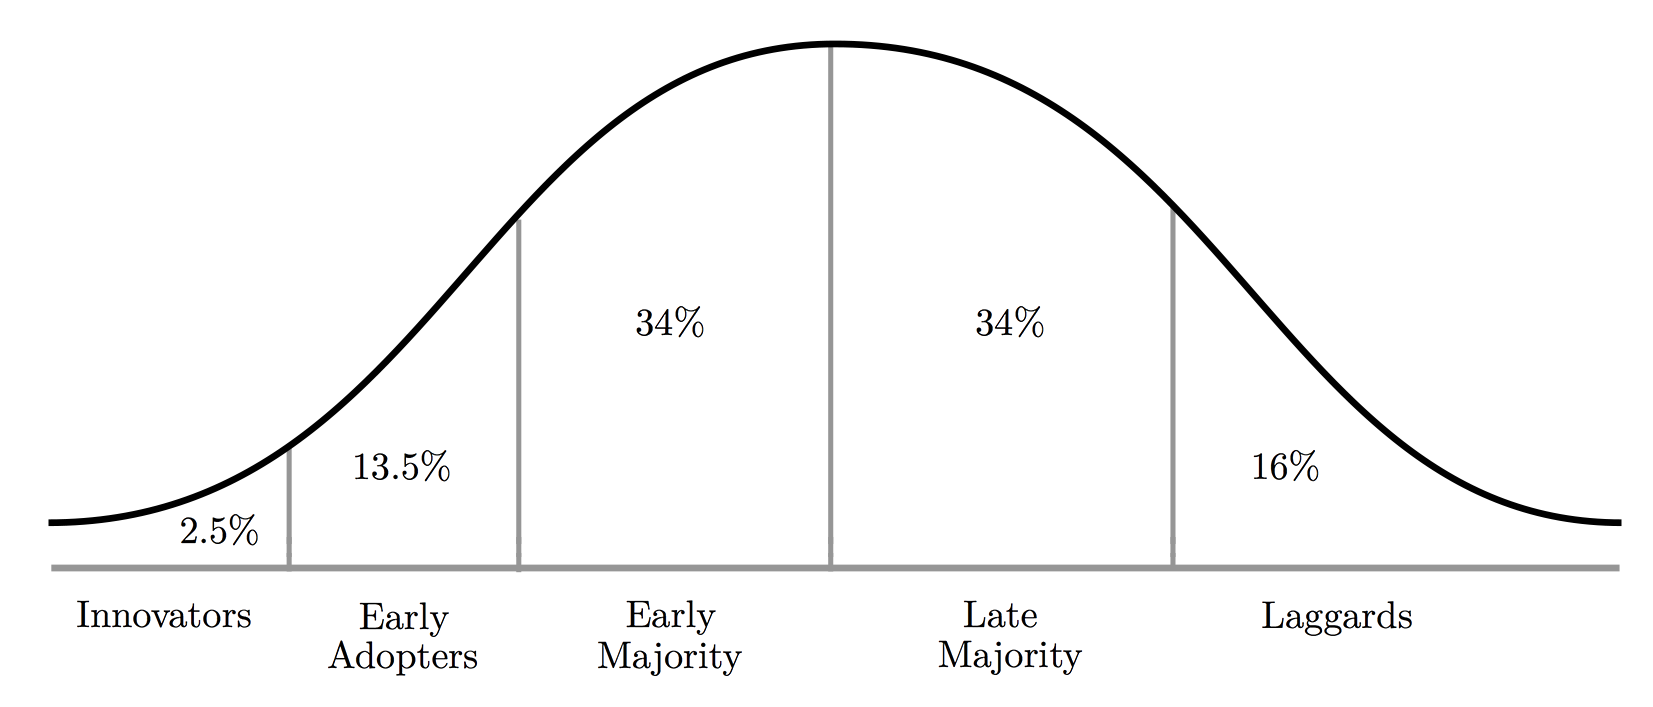
\includegraphics[width=0.8\textwidth]{Innovation_Diffusion}
  \caption{The diffusion of innovation across different adoption groups. (modified from \cite{Rogers1983})}
  \label{fig:Innovation_Diffusion}
\end{figure}

Whether or not an individual adopt an innovation and its affecting factors are conceptualized by Rogers in the \textit{innovation decision process} \cite{Rogers1983}. The process describe the individuals first contact and knowledge of the innovation, to the decision to adopt or reject, to implementation of the new idea, and to confirmation of this decision. This process contains five main steps: \begin{enumerate*}[label=(\(\arabic*\))]
  \item knowledge,
  \item persuasion,
  \item decision,
  \item implementation and
  \item confirmation.
\end{enumerate*}

\textit{Knowledge} occur when the individual first hears about the innovation's existence and when they gain understanding how it works. Rogers discuss three different types of knowledge for adoption; awareness-, "how-to"- and persuasion- knowledge. These types of knowledge may be required by actively seeking information about the innovation, but only after first being exposed to the innovation through an external source passively. After gaining \textit{awareness-knowledge} about the innovation, the information seeker may ask questions such as "What is the innovation", "How does it work?" and "Why does it work?". Awareness knowledge motivates the individual to seek "how-to" knowledge and principles knowledge. \textit{How-to knowledge} consists of the information required to use the innovation properly. Complex innovations require more how-to knowledge for proper adoption than less complex innovations, and thus are harder to adopt for the individual. \textit{Persuasion knowledge} is about understanding the underlying technology behind the innovation. For example, understanding biology and plant growth which underlie the innovation of fertilizer. The usage of an innovation without understanding the underlying concepts are usually possible, but the risk of misuse is greater.

\textit{Persuasion} occur when an individual form a favorable or unfavorable attitude toward the innovation. When this occur, the individual may think about the idea in terms of applying the innovation to his or her present or close future. At this stage, the person may ask questions such as "What are the innovation's consequences?" and "What will its advantages and disadvantages when I apply it in my situation?". The information gathered to answer these questions may be scientific, but most peers reach out to friends or people who have used the innovation before. When someone like ourselves tell us about the positive impact of the innovation we are more likely to adopt it ourselves.

\textit{Decision} occur when the individual engage in activities which will either lead the person to either adopt or reject the innovation. This means for most individuals to try out the new innovation at least partially. This time period as they apply the innovation is often part of the decision to adopt, and its important during this time to decrease the uncertainty of the value to the possible adopter. An accessible trial period of the innovation, e.g. a free sample or free time period, are generally adopted more rapidly compared to an innovation that must be adopted or rejected in its entirently. It is important to remember though that

\textit{Implementation} occur when an individual has decided to adopt the innovation and puts the innovation into use. All stages prior to the stage of implementation has been mostly a mental exercise for the individual, while the implementation stage involves a change of behavior. Even though the the person has decided to adopt the innovation, it is another thing to actually put it into practice. When they reach this stage, the individual may still have uncertainties about the consequences of the innovation. At this stage the individual will ask questions such as "Where do I obtain the innovation?", "How do I use it?" and "What operational problems may I face with the innovation?". The entirety of the implementation stage may continue for a lengthy period of time, but it will eventually reach a point where its either put into regular use or get exchanged with another new innovation.

The \textit{Confirmation} stage continue after the Implementation stage, and will continue for an indefinite period of time. At this stage the individual seek reinforcement that their decision to adopt was correct, and if the individual find conflicting messages about the innovation they may reconsider their decision. If the individual find information that he or she should not have adopted the innovation, they will experience \textit{dissonance}. Dissonance occur when new information become known to an individual which are conflicting with their current knowledge, opinion or behavior. The feeling of dissonance is uncomfortable to the person in question, and he or she will try to reduce it by changing their beliefs, attitude or knowledge. In the case of the confirmation stage, the person may avoid dissonance by only seeking information that only will support and/or confirm their decision to adopt. Contrasting information may still reach the individual which may make him or her doubt their decision to adopt.

\textit{Discontinuance}

\subsection{Accommodation}
% Accommodation Ge användare de verktyg de behöver för att lyckas. Implicit innebär dessa verktygen att de är användarbara också. Mentala modeler osv. Designa för användning med context.
Accommodation is the act of giving the users the tools they need to be able to succeed \cite{Bradt2009}. For the users to efficiently use the tools given, we have to understand their behavior; how they reason and learn. We discuss the theory of mental models and how us humans perform tasks.

\subsubsection{Behavior}
% similar to http://repository.cmu.edu/cgi/viewcontent.cgi?article=1045&context=hcii
Rasmussen \cite{Rasmussen1983} has identified three typical levels of performance. \textit{The skill-based behavior} represent the subconscious actions and activities which we perform on a "smooth, automated, and highly integrated patterns of behavior". This level of performance is based on a simple feedback loop, where a stimuli facilitate a motor output. \ignore{Provide example of this}

\textit{Rule-based behavior} are patterns of behavior which emerge from previous and similar actions performed in a previous similar occasion. The user acts in a goal-oriented way where the user tries to achieve a goal, which is usually not explicitly stated, with the rules that has empirically evolved through previous successful experiences.

The main differences of skill-based and rule-based behavior is that the person may not consciously be aware of the actions the user perform when performing actions on a skill-based level, and may not be able to recollect why such an action has been taken. The higher level rule-based actions are generally based on "explicit know-how, and the rules used can be reported by the person".

The third, and final level of performance as Rasmussen \cite{Rasmussen1983} has identified, is \textit{knowledge-based}. Knowledge-based performance is used during situations that the user is not familiar with, and where any know-how or rules cannot be used from previous experiences. Rasmussen \cite{Rasmussen1983} states that "In this situation, the goal is explicitly formulated, based on an analysis of the environment and the overall aims of the person. Then a useful plan is developed-by selection-such that different plans are considered, and their effect tested against the goal, physically by trial and error, or conceptually by means of understand the functional properties of the environment and prediction of the effects of the plan is considered." At this level of abstraction, the user represent the system in an internal construct called \textit{mental model}.

These three levels of performance are similiar to the types of user-product interactions identified by Forlizzi \cite{Forlizzi2004}; \textit{Fluent}, \textit{Cognitive} and \textit{Expressive} interaction.

\begin{description}
  \item[Fluent interactions] between a user and product are performed mostly automatically and do not compete for the users limited attention
  \item[Cognitive interactions], on the other hand, focus on the product and acquire most of the users attention. When users utilizing this level of interaction between themselves and a product it can result in expanded knowledge, confusion or cognitive error if the product does not work as the users expect. Cognitive experiences often result in some sort of change within the user (such as acquired skill or task award).
  \item[Expressive interaction] help the user form a relationship to the product, or some aspect of it. Through expressive interaction the user can change, modify and/or personalize the product to create a better fit of the product in the users life. These interactions can usually be expressed by the user as stories where additional value is added by the user
\end{description}

\subsubsection{Flow}
Flow was first conceptualized by Csikszentmihalyi as a mental state of "peak enjoyment, energetic focus, and creative concentration experienced by people engaged in adult play" \cite{Csikszentmihalyi1975}. Research since about this subject has been to understand this phenomenon of intrinsically motivated activity that exceeds that extrinsic good that might result from the activity.

The state of being in flow has been described with the following characteristics by some interviewees \cite{Nakamura2005}:

\begin{itemize}
  \item Intense and focused concentration on a particular task
  \item Hightened awareness of applications
  \item Loss of social awareness
  \item Superior sense of control of one's own actions
  \item Distortion of temporal experience
  \item Experience the activity as intrinsically rewarding rather than extrinsically
\end{itemize}

Being in the flow itself is intrinsically rewarding, and the individual who has achieved this heightened state of performance will seek to replicate the experience. As people get better and better executing a task, the challenge of the task gets lessened and is not as involving as before \cite{Nakamura2005}. In order to continue experiencing flow for a particular task, they must actively identify more complex challenges.

Staying in flow requires that the attention is held at the equilibrium of action opportunities and capabilities. If the task at hand is more challenging than the person is capable of the person is most likely to experience anxiety, while if the capabilities of the person are greater than the task requires the person will feel boredom. See figure \ref{fig:Flow-1} for representation of this orignal flow model.

\begin{figure}[h]
  \centering
    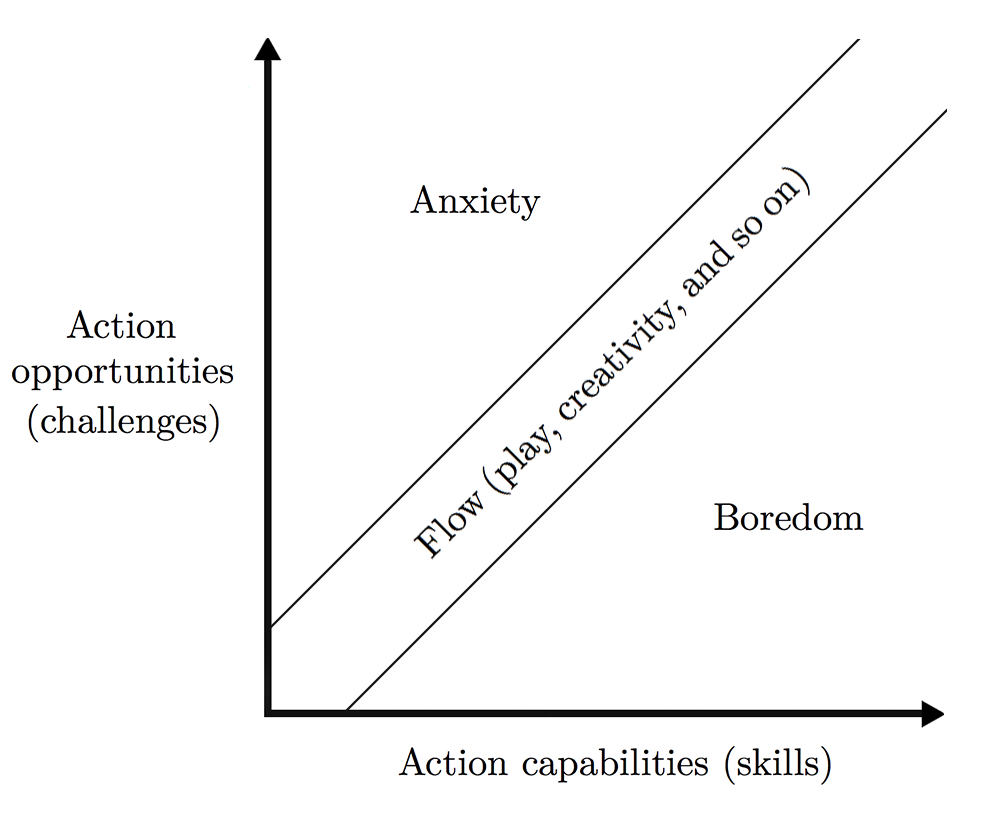
\includegraphics[width=0.8\textwidth]{Flow1}
  \caption{The original model of flow theory. (modified from \cite{Csikszentmihalyi2000})}
  \label{fig:Flow-1}
\end{figure}

Since the development of the original flow model (see figure \ref{fig:Flow-1}), further research has developed the model into a more detailed map with eight categorization instead of three. The eight categorizations are further devided into the amount of challenge for the task and intensity of experience in the form of concentric rings.

\begin{figure}[h]
  \centering
    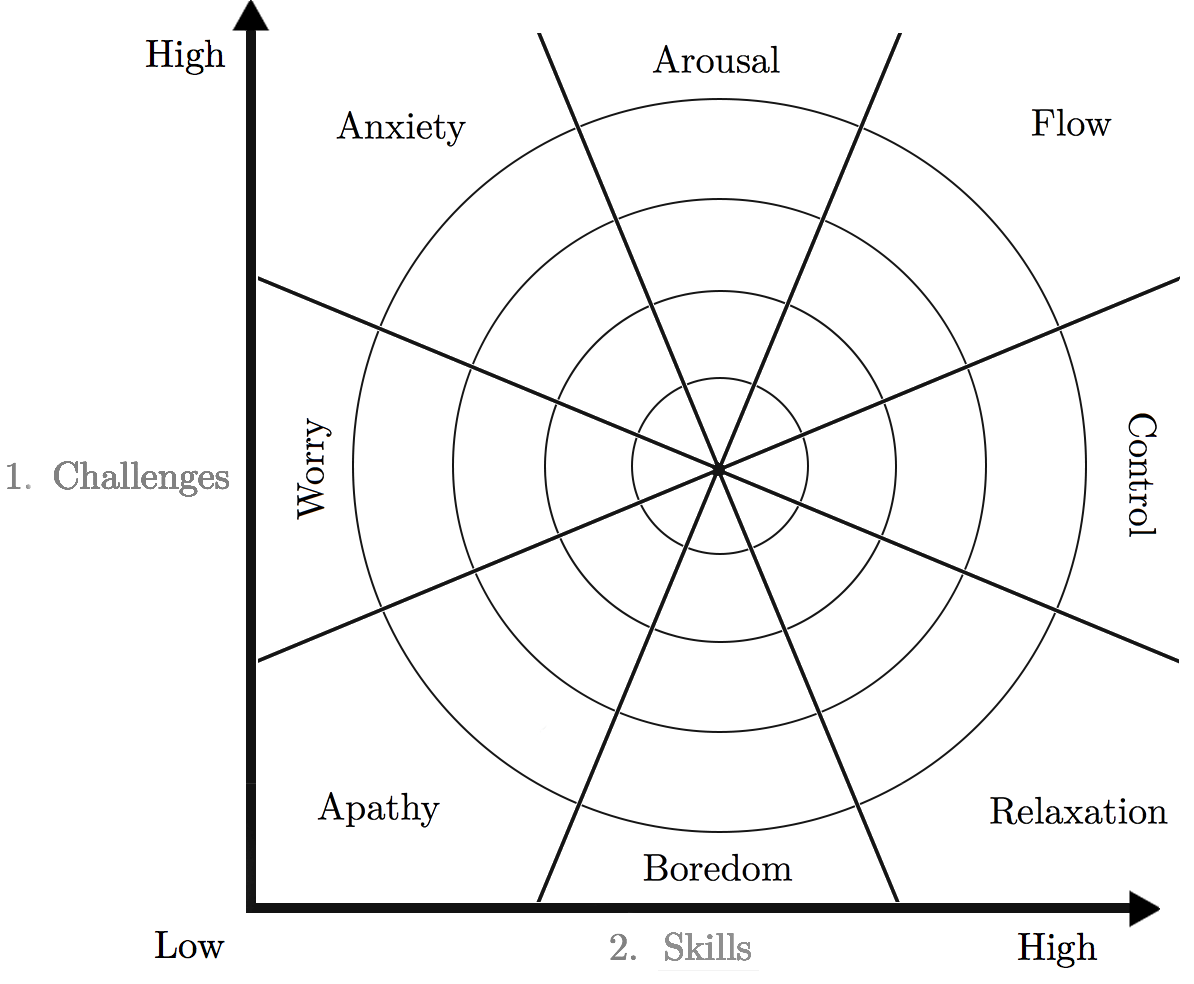
\includegraphics[width=0.8\textwidth]{Flow2}
  \caption{The current model of flow theory. (modified from \cite{Csikszentmihalyi1997})}
  \label{fig:Flow-2}
\end{figure}

\ignore{\url{http://journals.sagepub.com.proxy.ub.umu.se/doi/pdf/10.2190/UJ04-T5YB-YFXE-0BG2}}

\subsubsection{Keller's motivational design}
\ignore{\url{http://journals.sagepub.com.proxy.ub.umu.se/doi/pdf/10.2190/UJ04-T5YB-YFXE-0BG2}}
% Flytta till Acceleration kanske?
\ignore{\url{https://books.google.se/books?hl=sv&lr=&id=N_MVUyHxnkcC&oi=fnd&pg=PA383&dq=Keller’s+motivational+design+theory&ots=GLcChGLCS-&sig=Db7O30a_Y-9U88H7lueDI-lQVDE&redir_esc=y#v=onepage&q=Keller’s%20motivational%20design%20theory&f=false}}

\subsubsection{Mental model}
A common concept in the field of cognitive psychology is the concept of \textit{mental models}. Mental models was first introduced by American philosopher Charles Sanders Peirce, where he argues that humans reason by a process which
"...examines the state of things
asserted in the premises, forms a diagram of that state of things, perceives in the parts of that diagram relations not explicitly mentioned in the premises, satisfies itself by mental experiments upon the diagram that these relations would always subsist, or at least would do so in a certain proportion of cases, and concludes their necessary, or probable, truth." \cite{Pierce1974}

This was further elaborated by the psychologist Kenneth Craik who state that humans construct "small-scale models" of external reality \cite{Craik1967}. These mental models enable us to use past events to be able to react to present events and anticipate future events, to reason, and to understand our environment. Since Craik's contributions, cognitive psychologist has argued that mental models are formed through current and general knowledge, perception and imagination \cite{Johnson-Laird2001} \ignore{Find some more citations to support this claim}. In the field of Human-Computer Interaction (HCI) mental models has sometimes been used interchangeably with cognitive and conceptual models, and their difference and usage might be confusing as \cite{Staggers1993} concludes. For the purpose of this paper, we will be using Norman's \cite{Norman2013a} definition of conceptual and mental model, where he states that mental model needs to be consistent with the designers conceptual model. Mental models are the models made from experience, instruction and training which users interact through \cite{Norman2013a}, and the models become more mature as the user experience increase \cite{Barker1998}. Mental models of devices are created mostly through perceiving possible actions and its visible structures afforded by its interface \cite{Norman2013a}. The mental model of the user guide the users expectation of the application, and can guide the users navigation, planning of actions and contribute to the interpretation of interfaces feedback \cite{Jih1992}\ignore{not the actual source}. Mental models may act as both facilitators and inhibitors when learning, depending on the new information \cite{Cho1996}. When the user has acquired an adequate mental model of the structure and possible functions of the system the user is less likely to become disoriented \cite{Jih1992}, but if the user has trouble fitting new information into their current mental mode they experience frustration \cite{DApollonia2004}.

Norman \cite{Norman2013a} provide us with a seven-stage model which describe how users use interactive products.
\begin{enumerate}
  \item Forming the goal
  \item Forming the intention
  \item Specifying the action
  \item Executing the action
  \item Perceiving the system state
  \item Interpreting the system state
  \item Evaluating the outcome
\end{enumerate}

This model of actions help us describe how an user explore an interface \cite{}\ignore{Polson and Lewis, 1990}. This approximate model \cite{Norman2013a} is not consciously used by the user, but rather it tries to explain how we perform tasks. The model is cyclic, meaning that the user will experience multiple loops of the model as they explore an interface. The model is developed on the basis that human actions has two aspects; execution and evaluation. Execution is doing something which affect the world, and evaluation is the comparison if the world reached or got closer to a state which was desired by the user. These two aspects have their of stages of performance. The stages of execution involves forming the goal, which may be an abstract representation of what we want to achieve (get to work, eat dinner, pick a movie). The goal forms our intentions to perform an action, which constitutes in an action sequence to be executed to satisfy the intention. Finally in the stage of execution, the action sequence is executed upon the world and we reach the stages of evaluation. The first stage of evaluation is perceiving the systems state. The perception is then interpreted according to our expectations and finally compared to our intentions and goal. As the users try to finish their tasks, there are four critical points where user errors can occur, as identified by \cite{Shneiderman2004}:
\begin{enumerate*}[label=(\(\arabic*\))]
  \item users form an inadequate goal,
  \item users might not find the correct interface touchpoint because of a label or icon that does not sufficiently represent its corresponding action
  \item users may not know what action to perform to get a desired output and
  \item users get misleading feedback from the system
\end{enumerate*}

Getting the user to have a representative mental model of the system is key to any apps success

\subsubsection{Gulf of evaluation and execution}
% Expand this section.
The user initially start with an intention of achieving a goal, where the goal is often expressed in psychological terms. The system or interface

\subsubsection{Expectation-Confirmation Model}
The expectation-confirmation model (ECM) examine the cognitive beliefs and affects that influences one's intention to continue using information systems \cite{Bhattacherjee2001a}. The model stems from Expectation-confirmation theory (ECT) which has been widely used to study consumer satisfaction, post-purchase behavior and service quality control in general (\cite{Anderson1993} \cite{Oliver1981} among others). The process which consumers conclude their satifsaction or dissatisfaction of a product is by \begin{enumerate*}[label=(\(\arabic*\))]
  \item forming an initial expectation of the product or service before purchasing,
  \item they form a perception about the performance of the product after a period continued use,
  \item they compare their perceived performance with their initial expectation, and conclude whether or not their expectation has been confirmed,
  \item depending on the level of confirmation and expectation they achieve a certain level of satisfaction of the product.
  \item Finally, depending on the level of satisfaction the consumer decide whether or not to repurchase the product and continue its use. Dissatsfied users discontinue the use of the product.
\end{enumerate*}

The feeling of \textit{satisfaction} of a product has been defined as "the summary psychological state resulting when the emotion surrounding disconfirmed expectations is coupled with the consumer's prior feelings about the consumption experience." by \cite{Oliver1981}, while Bhattacherjee has defined it as "an ex post evaluation of the users’ initial trial experience with the service as is captured as a positive feeling, satisfaction, indifference or negative feeling (dissatisfaction)" \cite{Bhattacherjee2001}. Both definitions imply a that the state of satisfaction is based on the appraisal of expectation versus outcome, as expectation sets the bar for the customer to which the customer will compare the product to. A lower expectation and/or higher product performance lead to a greater level of confirmation, which dictates the customers satisfaction. A high expectation and/or low product performance lead to disconfirmation, dissatisfaction and an intention of product discontinuence.

According to the ECM, the person using an IS continually adjust their perception of the perceived usefulness about the IS as they acquire new information. The model proposes that perceived usefulness and confirmation are the leading factors that determine the willingness of IS continuance through satisfaction. As we can see in figure \ref{fig:ECM} confirmation also influence perceived usefulness.

\begin{figure}[h]
  \centering
    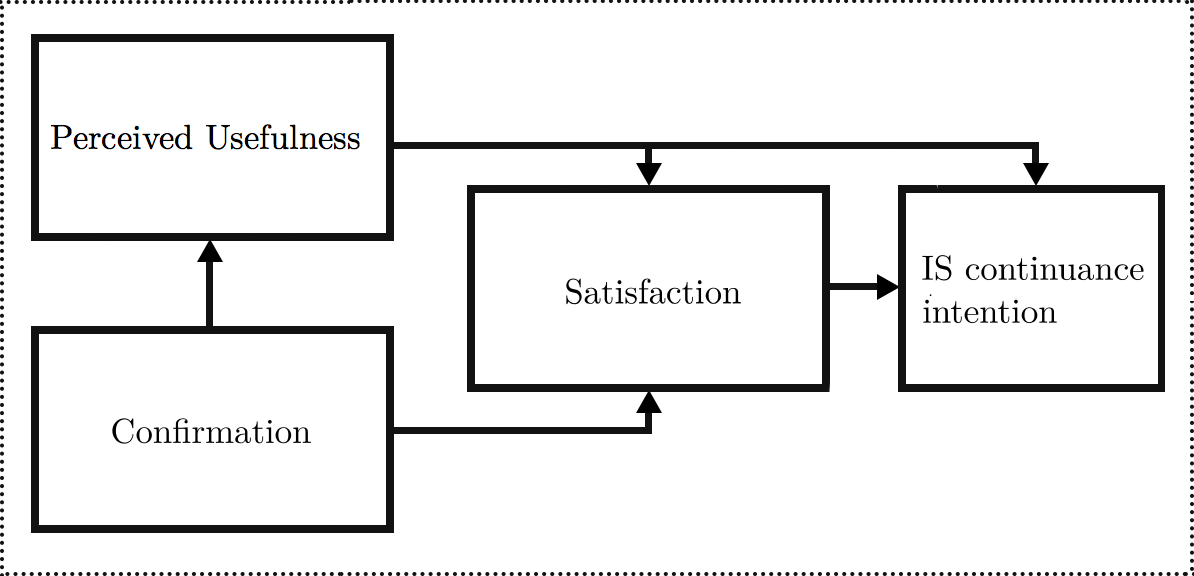
\includegraphics[width=0.8\textwidth]{ECM}
  \caption{Expectation-Confirmation Model (ECM). (modified from \cite{Bhattacherjee2001a})}
  \label{fig:ECM}
\end{figure}

\subsubsection{Learnability}
More often than not, "interface usage requires learning" \cite{Grossman2009}, and the growing number of  products which do not have any formal documentation need to be learned in a few minutes or risk being abandonded \cite{Bergman2000}. Even though there is plentiful of research regarding learnability, its definition is not widely agreed upon. The different definitions consider different scopes of learnability, e.g. Nielsen definition consider the initial learning curve of the user, and that a highly learnable system would be "allowing users to reach a reasonable level of usage proficiency within a short time." What "a reasonably level of usage proficiency" is relative to a "short time" is still unclear, and it leaves a lot to our own imagination. Schneiderman and Plaisant provide us with a more general applicable definition of "the time it takes members of the user community to learn how to use the commands relevant to a set of tasks" \cite{Shneiderman2004}. Schneiderman and Plaisant also discuss different aspects which they argue affect interface learnability, which is \textit{Retention over time}; How well is the user able to recall how to use an application after a specific time period? Retention may affect time to learn \cite{Shneiderman2004}.

\begin{description}
  \item[Time to learn] How long does it take for the typical user to learn the required actions to reach a goal?
  \item[Speed of performance] How long does it take to reach the main goals?
  \item[Rate of errors] How many user or interface errors occurs when the users perform the main actions?
  \item[Subjective satisfaction] Did the users have a positive experience using the interface?
\end{description}

Succeeding in each of these categories may be hard for the designer, and succeeding in one category may require tradeoffs in another. For instance, if we want to have a low rate of errors we may need to sacrifice speed of performance. The designer and project managers need to identify which of these categories will be most valued by the users \cite{Shneiderman2004}.

\ignore{\url{http://www.lawrence-najjar.com/papers/Principles_of_educational_multimedia_user_interface_design.html}}

The characteristics of the material to learn can significantly affect learning. From a psychological standpoint, the learning characteristics include the medium itself, physical structure, conceptual difficulty, and sequence \ignore{\cite{Bransford1978}}. The following text will discuss ways to improve learnabilty through the medium of the material.

Images seem to help the user learn information more effectively. For example, it has been found when testing recall that pictures of common objects had a higher success rate than their textual names \cite{Lieberman1965} \cite{Nelson1976} \cite{Paivio1969} \cite{Paivio1973}. This is not true though when the images represent similar object \cite{Nelson1976} or when they attempt to communicate abstract concepts such as "freedom" or "amount". The combination of images and textual words improves recall \cite{Paivio1973} and comprehension of text \cite{Levie1982}.

Nugent \ignore{\cite{Nugent1982}} got the highest levels of learning when she presented information as a combination of text and images or text and audio compared to the same content via text, audio or images alone. Leung \cite{Leung2009} has found that when using icons for interface functions, labeling them will help users correctly interpret the function. Similarly, a study by Wiedenbeck found that first time user had a best performance with label and icon-label interface, and icon-label had a higher perception of ease of use among participans than icon only and label only \cite{Wiedenbeck1999}.

Encouraging the user to elaborately learn the material through interactivity may improve learning \cite{Bower1970} \cite{Jacoby1979} \cite{Bosco1990}. An interactive user interface has found a significant positive contribution to learning \cite{Bosco1990} \cite{Fletcher1989} \ignore{\cite{Bosco, 1986; Fletcher, 1989, 1990; Stafford, 1990; Verano, 1987}} and retention of knowledge over time \ignore{\cite{Stafford 1990}}. It has also been found that user may learn the learning material faster and may have a better attitude to learning the material when they use an interactive instructional environment. \ignore{\cite{Bosco, 1986; Fletcher, 1989, 1990}}

More design principles are provided by \cite{Lohr2000} on how :

\begin{itemize}
  \item Make the difference between fore- and background as distinct as possible to help the user percieve the signals of the interface correctly.
  \item Help the user understand the hierarchy of instructional tasks by organizing interface elements into meaningful section of information
  \item Design and organize the interface elements into a coherent whole so that the learner has an overall idea of what the environment is like and what is expected of the learner
\end{itemize}

Interaction in itself does not necessarily help the user to learn. The interaction must be cognitively engaging and challenge the user \ignore{\cite{???}}.

Kristoffersen has identified four principles of learnability.

\begin{description}
  \item[Predictability]
  \item[Consistency]
  \item[Generalizability]
  \item[Familiarity]
\end{description}

\ignore{A small number of studies provide limited support for this design principle. Multimedia can help direct the learner's attention to relevant information and improve learning. For example, one study (Baxter, Quarles, & Kosak, 1978) asked adults in a shopping mall to "look over" a newspaper page that included a story with or without a large photograph. When asked questions about their recall of the newspaper story, the participants remembered more information when they saw the story with the photograph than when they saw the story without the photograph. It appears that the photograph got the participants' attention and caused them to read the accompanying story. Other researchers successfully used drawings (e.g., Paradowski, 1967; Tennyson, 1978), motion (Baek & Layne, 1988; Park & Hopkins, 1993), small "chunks" of textual and graphical information (Rieber, 1990b), and adjunct questions (e.g., McConkie, Rayner, & Wilson, 1973; Watts & Anderson, 1971) to focus the learners' attention.

However, getting a learner to pay attention to information does not necessarily mean that the learner will learn the information. For example, learners who are new to a field of knowledge may simply view a supplementary animation without trying to understand the information it shows (e.g., Reed, 1985). Also, irrelevant media, such as unrelated pictures (e.g., Levie & Lentz, 1982) or motion (Park & Hopkins, 1993) may distract learners and actually decrease learning performance.}

\ignore{Processing tasks that encourage learners to integrate the information they are studying seem to improve learning. Several studies (e.g., Anderson & Biddle, 1975; Frase, 1975; Reder, 1979; Rothkopf, 1966) found that periodically asking learners to answer questions about the information they had just reviewed led to improvements in learning performance. Tasks that do not encourage learners to integrate the information may actually worsen learning performance (e.g., Stein & Bransford, 1979; Stein, Morris, & Bransford, 1978).}

\subsubsection{Feedback}
When the user explores an interface and learn it, feedback "is an important aspect of effectively designed learning environments and should occur continuously and unobtrusively as an integral part of the instruction" (Bransford, Brown, \& Cocking, 1999) \url{https://www.researchgate.net/profile/Chun-Han_Chiang/publication/220374484_An_Individualized_e-Reading_System_Developed_Based_on_Multi-representations_Approach/links/0deec53488a7b809f8000000.pdf#page=116}
Norman \cite{Norman2013a} tells us to provide continuous feedback and clear information about the results of the users actions.

\subsubsection{Human-Computer Dialogue}

If the conceptual model is not clearly communicated to the user and is not properly corrected through computer-human dialog, the user will have trouble performing the tasks they've set out to solve their problem. Studies of blame \ignore{Find these studies}, or \textit{attribution}, has shown that when a fault occurs in a system, the person in question is more likely to attribute the error to system than their own. Similarly, when fortune occurs to a person they are likely to attribute the fortune to their person and intelligence.

If the users mental model is not consistent with the conceptual model provided by the designer, the users mental model can be modified through a \textit{computer-human dialog}

The communication between a user and a computer-based system is through a \textit{user-computer dialogue} \cite{Foley1996}, where the dialogue is communicated through a language of inputs and outputs. Similarly to regular human-to-human conversation, we may provide feedback if something is misunderstood or help the other person finish a sentence. The same is true for human-to-computer communication, where feedback is used to reinforce or discourage the users action, making the user adjust his or her mental model of the system.

The area of psychology that focuses on the environmental determinants of learning and behavior.

\subsubsection{Memory}

%% DESIGN
\subsubsection{Cognitive load}
The larger the amount of available information is given to the user from an interface, the more likely it is for the user to fall under the pressure of excessive cognitive load. According to \cite{Jih1992}, the user of an interface has to endure three different types of cognitive load; the content of the application, the application structure and the responses and feedback given by the interface. Schneiderman et al. state that "Providing excessive functionality ... is also a danger, because the clutter and complexity make implementation, learning, and usage more difficult".

\subsubsection{Affordances / Signals}

\subsubsection{Incidental and Informal learning}
Incidental learning is unintentional or unplanned learning that results from performing activities \cite{Kerka2000}; activities which primary objective is not to acquire knowledge but to progress while pursuing a goal. As Kerka \cite{Kerka2000} has identified in her literature review of incidental learning, incidental learning may occur "through observations, repetition, social interaction, and problem solving; ...; from mistakes, assumptions, beliefs, and attributions; or from being forced to accept or adapt to situations". Incidental learning at this time was discussed in the context of workplace learning, but as \cite{Marsick2001} conclude, this type of learning happen through "everyday encounters while working and living in a given context". Jones et al. \cite{Jones2014} has drawn the conclusion that this type of learning is particularly suited for smartphone use.

\subsection{Assimilation}
\label{sec:assimilation}
% Assimilation Göra så att de är välkomna i sitt nya område, och om appen erbjuder ett community, att de känner sig välkomna där. Language, welcome
Assimilation is helping the user feel welcome in their new community and environment so that they can accomplish their tasks together \cite{Bradt2009}.

\subsubsection{Community}

A community is no longer defined as a physical space where relationship between people happen face-to-face, but rather as a set of relationships where people interact socially for mutual benefit. This broader definition is required to accommody \textit{online communities}, where a online community is defined as a social network that uses computer support as the primary basis of communcation among members.  In online communities, potential members are quick to evaluate the community and decide whether or not they want to be a part of it. Community designers want to present the user with an accurate representation of the community and what is expected of the user to be a part of it.

Traditionally, "off-line" groups create entry barriers to make sure that people who join the group are people who are willing to commit and will belong in the group. The nature of the entry barrier may be subjective (submitting a work sample to join an art school) or objective (intelligence test score to join Mensa). Joining a group with an entry barrier, subjective or objective, require some level of commitment from potential members. The entry barrier may be to simple write a signature on a sign up form or pay a fee to join a gym. These barriers exist with online communities as well, e.g. to join dribbble you need an invite from another member of the community.

It has been found that there is an correlation between the difficulty of an entry barrier and the people's level of commitment to a group once they have passed the barrier \cite{Aronson1959}, which has been verified by Drenner et al \cite{Drenner2008} on a movie recommendation online community where they found that users where four times as likely to contribute to the community if they imposed a higher barrier of entry.

Discuss social media and its implications to feeling welcome etc...
\subsubsection{Design}
Discuss different platforms and their interface design language, and how being familiar with a design is good...

\ignore{
Moreover, cultural traits have also been identified as one of the most important
factor that impacts users’ perceptions towards different features of IT and mobile
services (Hiller, 2003)
Cultural differences have undeniable effect on
organizations and behaviour (Sarala, 2010)

First impressions matter. In online communities, potential members
quickly evaluate the community and decide if they want to
participate in it. And community designers want to present potential
members an accurate picture of the community, including what
is expected from members.
% https://pdfs.semanticscholar.org/6a58/9a768f9e56fb06e9aa9a975e6fca74644f03.pdf
% https://pdfs.semanticscholar.org/75e9/749b45cb3fb5dcfb6e7e918513098ad4d60c.pdf
}

\subsection{Acceleration}
% http://www-tandfonline-com.proxy.ub.umu.se/doi/full/10.1080/0144929X.2010.489665?scroll=top&needAccess=true
Acceleration is helping the user accomplish tasks faster and better \cite{Bradt2009}.

\subsubsection{Mental model maintenance and building}
Acceleration and the improvement of user proficiency is usually accomplished when the user is getting familiar with the interface and the app, and an adequate mental model has been built. When new features are introduced that might help the user accomplish a task faster, the user will initially rely on the mental model they currently have to make sense of the new feature \cite{Orlikowski2000}. New information is fed back to their mental model as the users explore the new features, and two subprocesses may occur: \textit{mental model maintenance}, where the users try and incorporate the new feature into their existing mental model, and \textit{mental model building} where the users reconstruct the mental model to include the new information and knowledge \cite{Vandenbosch1996}. Zhang et al. \cite{Zhang2011} draw the conclusion that when mental model maintenance occur, the user can reaffirm their previous mental model and their existing pattern of usage can continue with much change. Mental model maintenance will therefore lead to a more favourable view of the new feature, and learning it will take less effort. Mental model building, on the other hand, requires modifying, restructuring and sometimes requires entirely discarding previous mental model \cite{Vandenbosch1996}. Mental model building occurs most often when functionality is replaced, whereas mental model maintenance most often occur when functionality is extended or added. Mental model building requires the aid of the application and interface to correct the faulty mental model, such as feedback from actions and information that contrasts with current thinking \cite{Hsu2011}.

\ignore{
%% PROBLEMS
\subsection{Human interaction with smart devices}
\subsection{Mobile smart devices}

\subsubsection{Human interaction with mobile smart devices}
Identifying the context of use is the starting point of human-centered des

In a study where they examined reviews of mobile applications on the iOS operating system, interface design was one of the five most common complaints \cite{Khalid2015}. It was superseded by \textit{Functional error}, \textit{Feature Request}, \textit{App crashing} and \textit{Network Error}.
Designing for mobile devices such as smartphones introduce a number of different unique problems such as small screen sizes, limited connectivity, limited battery and restricted set of available inputs \cite{Zhang2005}. One of the biggest challenges is to consider the context of which they are used in \cite{Zhang2005} \cite{Harrison2013} \cite{Korhonen2010}. Korhonen et. al \cite{Korhonen2010} has identified eight possible contextual factors one has to consider when designing for mobile devices;
\begin{description}
  \item [Environment Context] The environment context describe the surrounding area of the user and the other entities it contains which can affect the user directly or indirectly.
  \item [Personal Context] The personal context describe both the physiological characteristics and attributes (pulse, blood pressure and hair color etc), and the mental attributes of the user (mood, expertise and stress). Mental attributes are most often considered when designing for the context of use.
  \item[Task Context] The task context describe the events, actions and activities the user is currently engaged in. This context also describe if the use of a device is a primary or secondary task.
  \item[Social Context] Expand
  \item[Spatio-Temporal Context] Expand
  \item[Device Context] Expand
  \item[Access Network Context] Expand
\end{description}
While modern smart phones are packed with a lot of functionality (GPS navigation, voice and data communication, multimedia consumption, gaming) their small form factor limit the possible input and outputs. The two primary means of input supported by these kind of devices are
\begin{enumerate*}
  \item Touchscreen and
  \item Sensors
\end{enumerate*}

\subsection{Memory}
\subsection{Language}
\subsection{Interface design}
To be able to effectively use the intrinsic motivation of the user, it is
}

\section{Best practice evaluation}
\label{sec:best_practice_evaluation}

To understand the industry and what techniques they deploy to onboard users we have done an analysis of the applications \textit{dots}. All tests were performed on an iPhone 6s+.

\subsection{Dots}

Dots is a puzzle game on iOS and Android where you connect dots together. They use an \textit{interactive tutorial} where the user is introduced to mechanics of the game.

\begin{figure}
\centering
\captionsetup{format=multiline,font=footnotesize}
\begin{minipage}{.33333\textwidth}
  \centering
  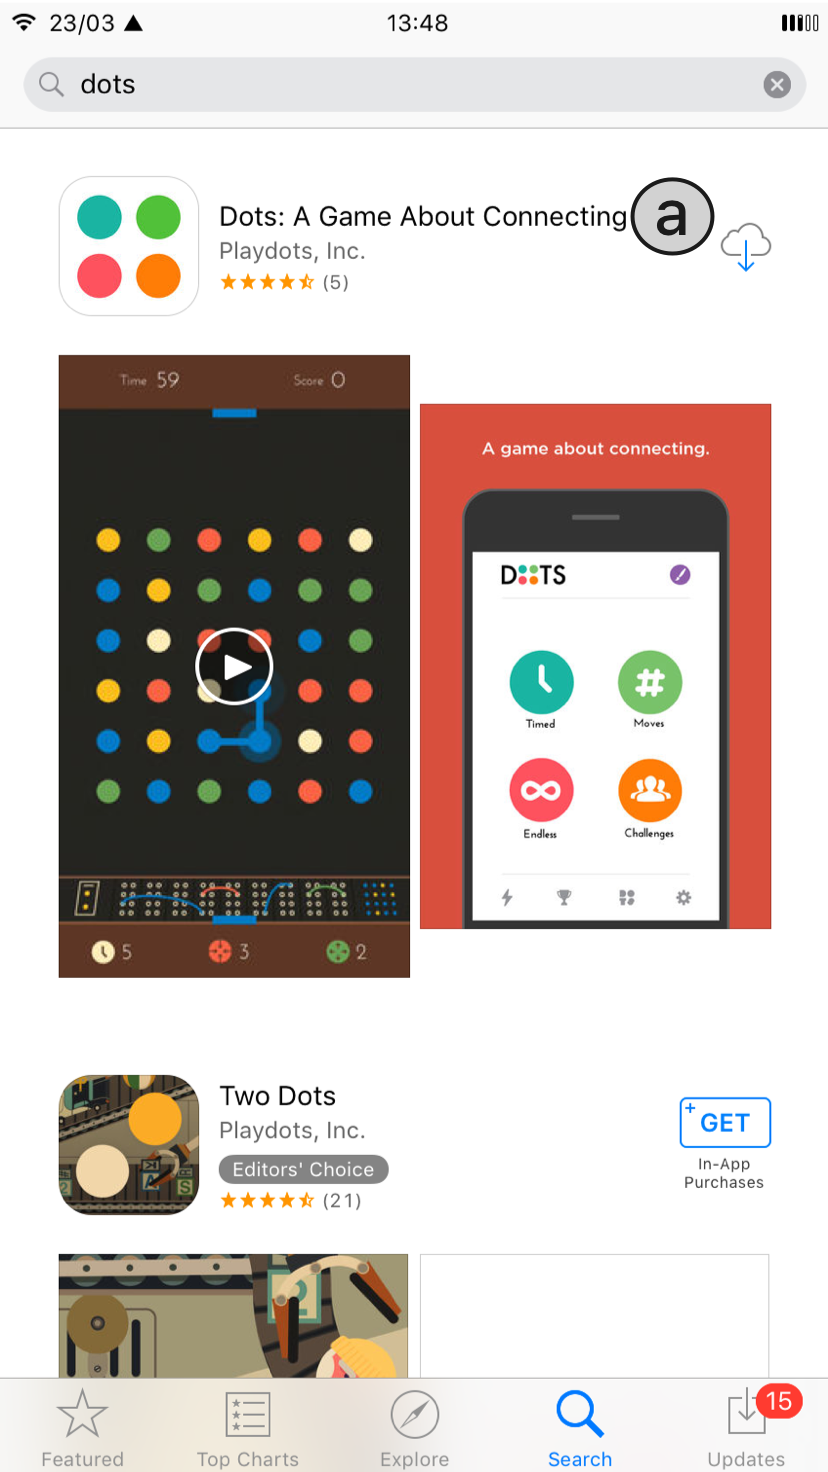
\includegraphics[width=.8\linewidth]{dots/1:1.png}
  \captionof{figure}{\\Dots in "App Store"}
  \label{fig:1:1}
\end{minipage}%
\begin{minipage}{.33333\textwidth}
  \centering
  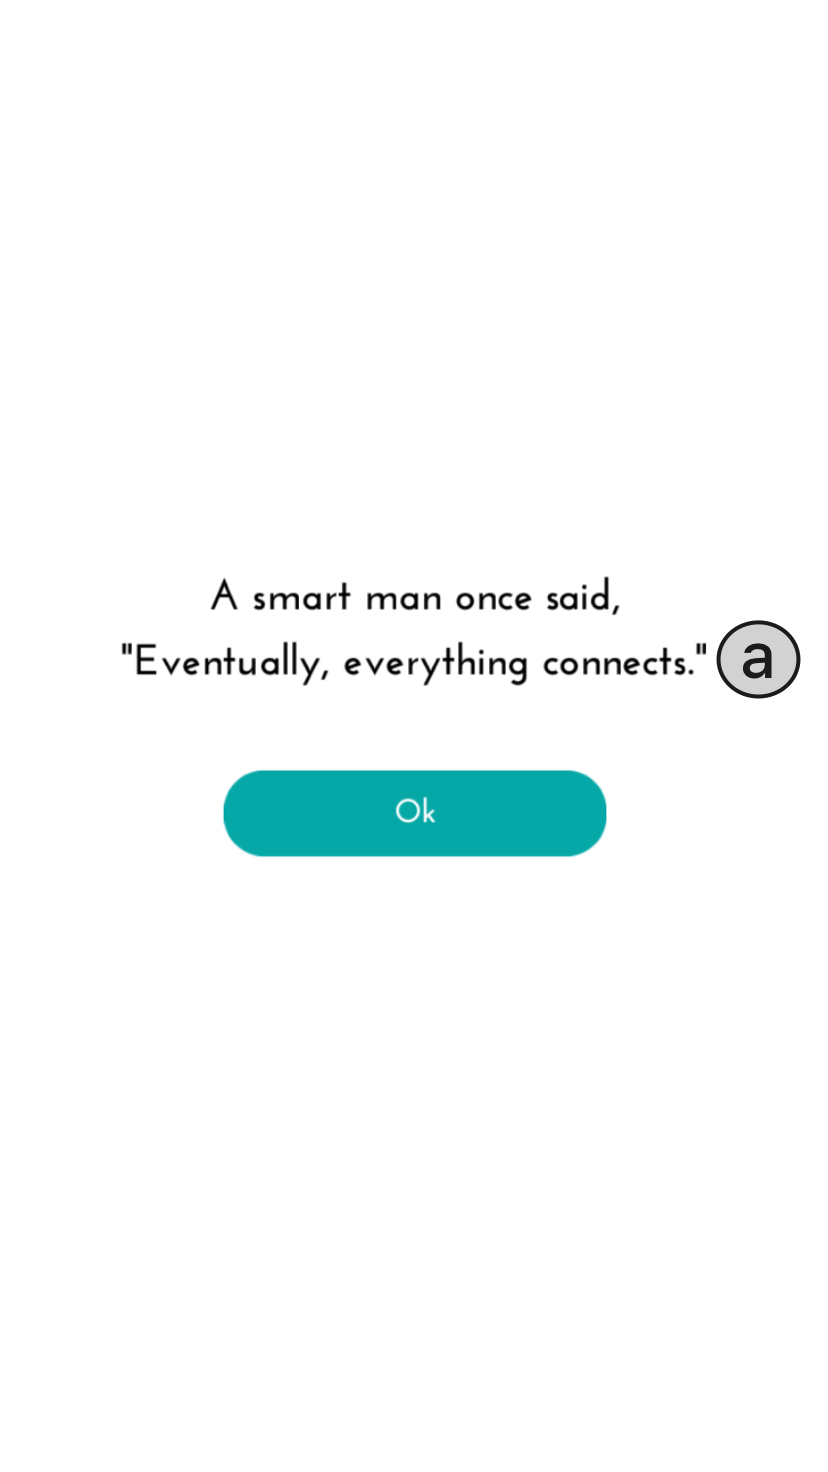
\includegraphics[width=.8\linewidth]{dots/1:2.png}
  \captionof{figure}{\\The first screen}
  \label{fig:1:2}
\end{minipage}%
\begin{minipage}{.33333\textwidth}
  \centering
  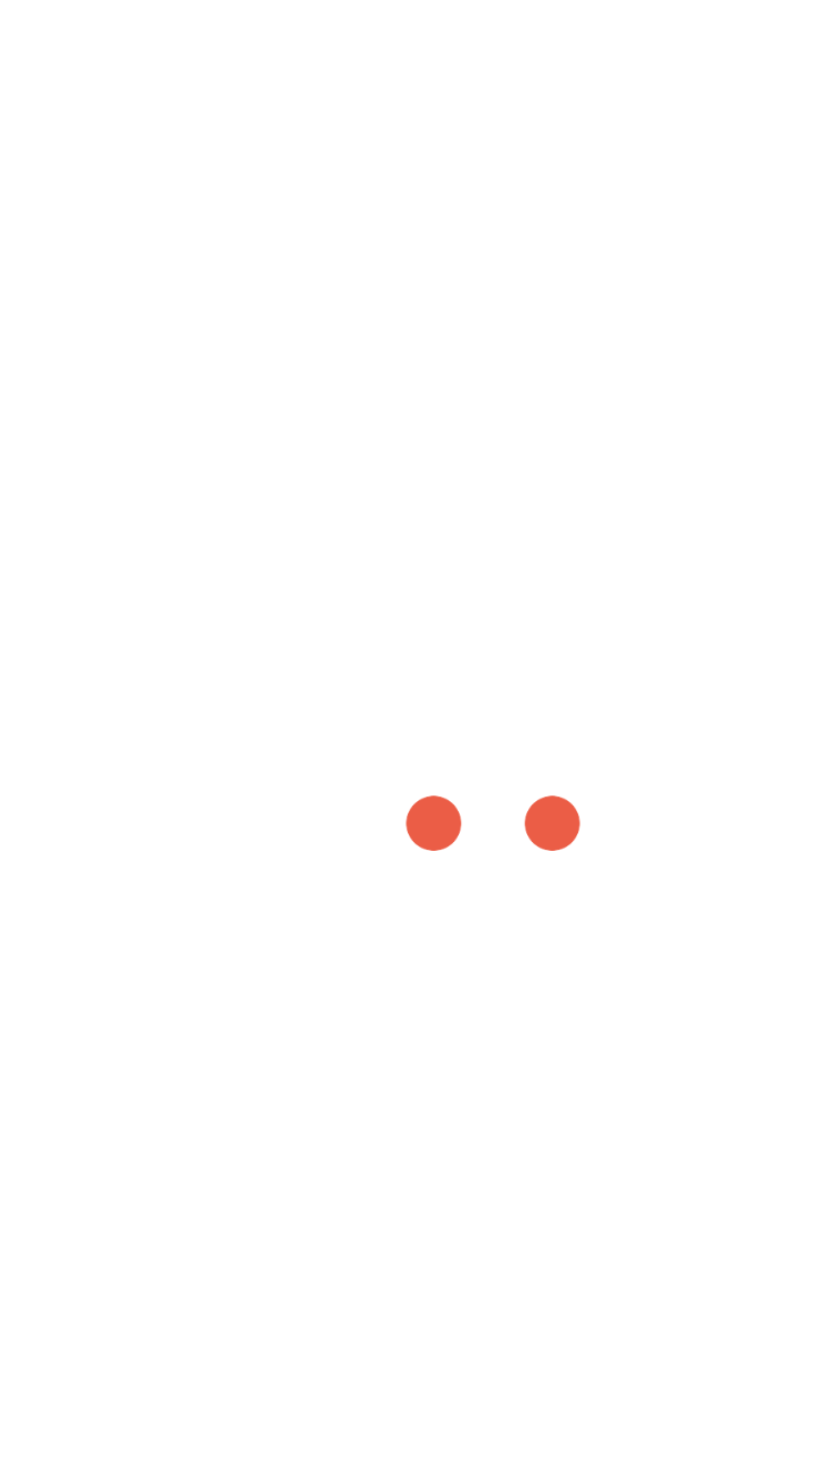
\includegraphics[width=.8\linewidth]{dots/1:3.png}
  \captionof{figure}{\\Start of the tutorial}
  \label{fig:1:3}
\end{minipage}
\end{figure}

The title hints to the user that the game is about connecting dots (Figure \ref{fig:1:1} (a)), which is further verified by the first screen when you open the app (Figure \ref{fig:1:2} (a)). The quote leaves out who said "Eventually, everything connects". After pressing OK in Figure \ref{fig:1:2} we are presented with two red dots. The only possible action here is to connect the two dots (Figure \ref{fig:1:4}).

\begin{figure}
\centering
\captionsetup{format=multiline,font=footnotesize}
\begin{minipage}{.33333\textwidth}
  \centering
  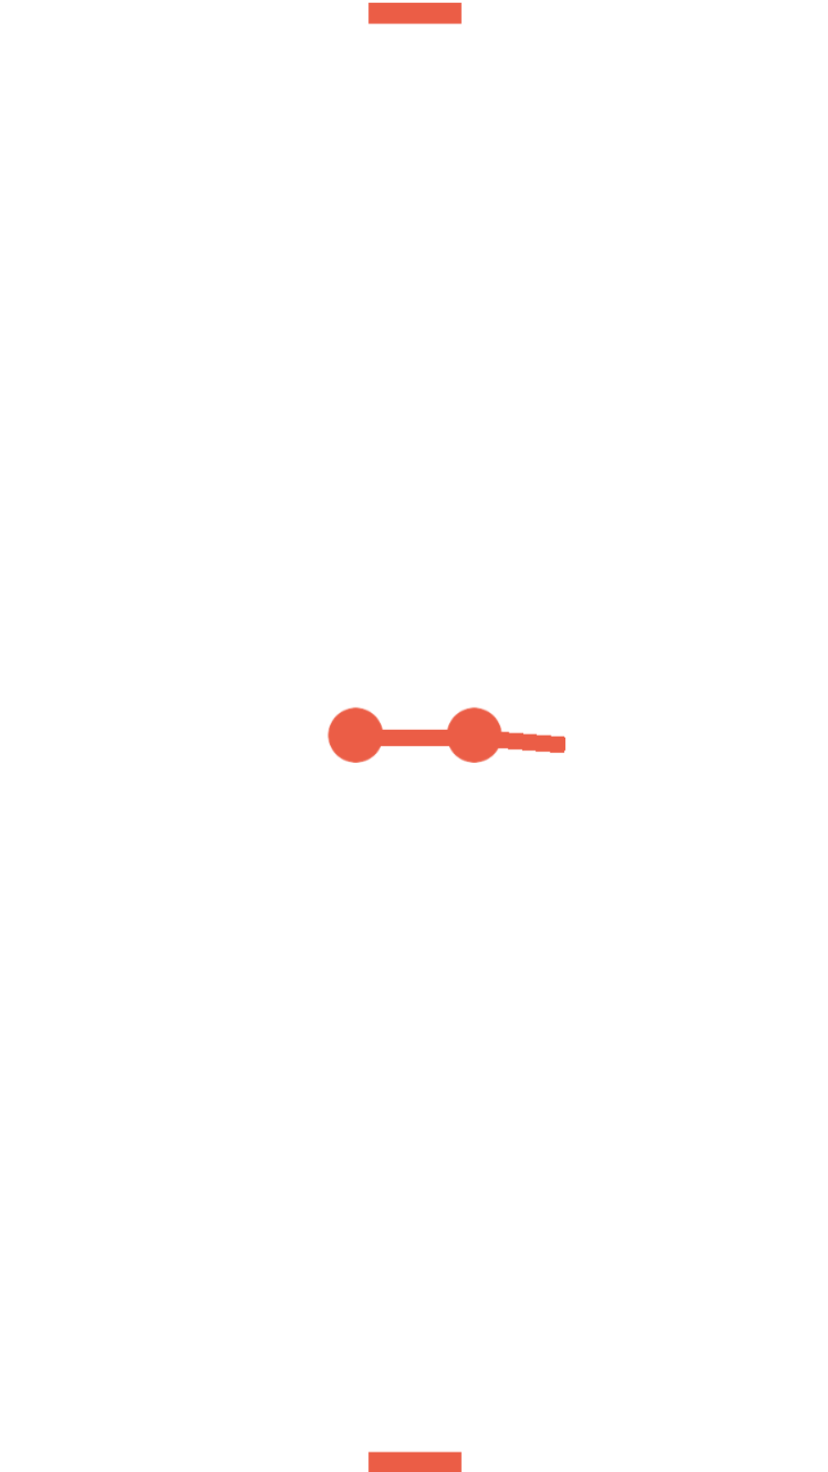
\includegraphics[width=.8\linewidth]{dots/1:4.png}
  \captionof{figure}{\\Connecting the two dots}
  \label{fig:1:4}
\end{minipage}%
\begin{minipage}{.33333\textwidth}
  \centering
  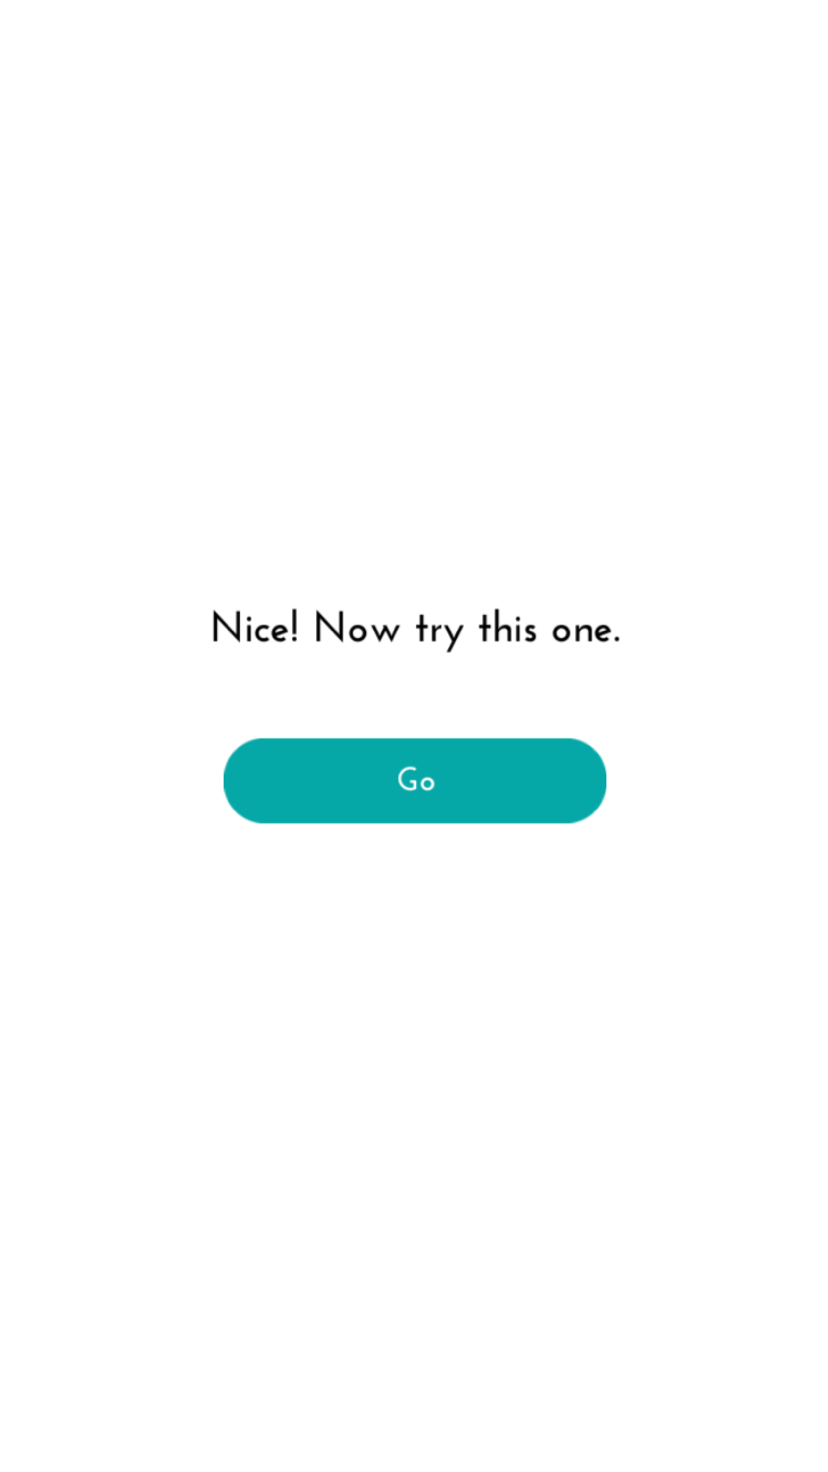
\includegraphics[width=.8\linewidth]{dots/1:5.png}
  \captionof{figure}{\\Positive reinforcement}
  \label{fig:1:5}
\end{minipage}%
\begin{minipage}{.33333\textwidth}
  \centering
  
\includegraphics[width=.8\linewidth]{dots/1:6.png}
  \captionof{figure}{\\Next challenge}
  \label{fig:1:6}
\end{minipage}
\end{figure}

We connect the dots by tapping, holding and dragging between them with one of our fingers. As we do this we can see a line forming at the top and bottom of the screen. As we release our finger we get some positive reinforcement that we successfully completed the task (Figure \ref{fig:1:5}). After pressing the button labeled "OK" we're presented with the text "Make a square" and four purple dots (Figure \ref{fig:1:6}). We know from before (Figure \ref{fig:1:4}) that we can horizontally connect dots, and we can now figure out that we can connect them vertically as well. We also now know that the dots can be of different colors.

\begin{figure}
\centering
\captionsetup{format=multiline,font=footnotesize}
\captionsetup{format=multiline,font=footnotesize}
\begin{minipage}{.33333\textwidth}
  \centering
  
\includegraphics[width=.8\linewidth]{dots/1:7.png}
  \captionof{figure}{\\Failing to make a square}
  \label{fig:1:7}
\end{minipage}%
\begin{minipage}{.33333\textwidth}
  \centering
  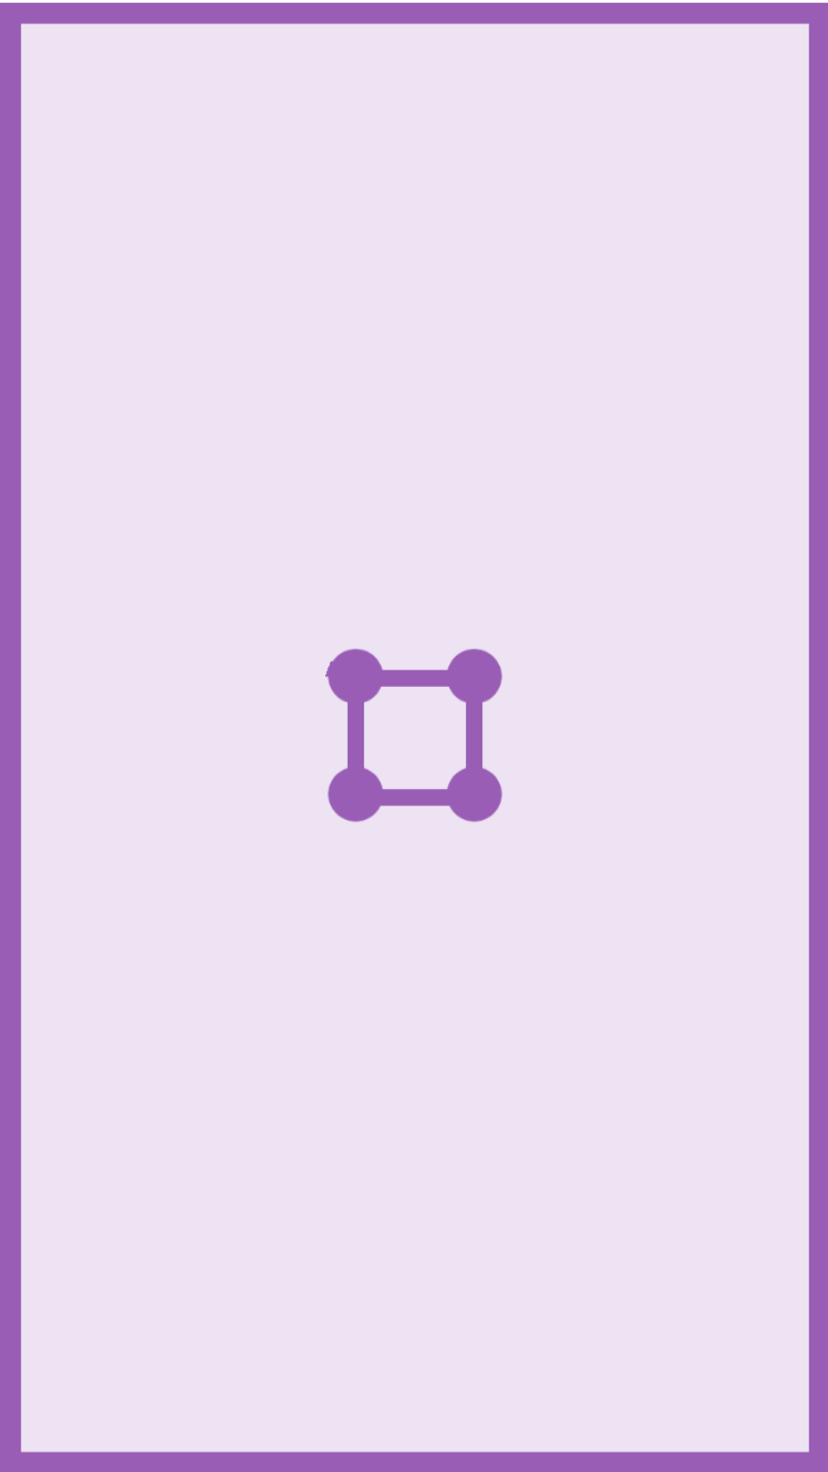
\includegraphics[width=.8\linewidth]{dots/2:1.png}
  \captionof{figure}{\\Making a square}
  \label{fig:2:1}
\end{minipage}%
\begin{minipage}{.33333\textwidth}
  \centering
  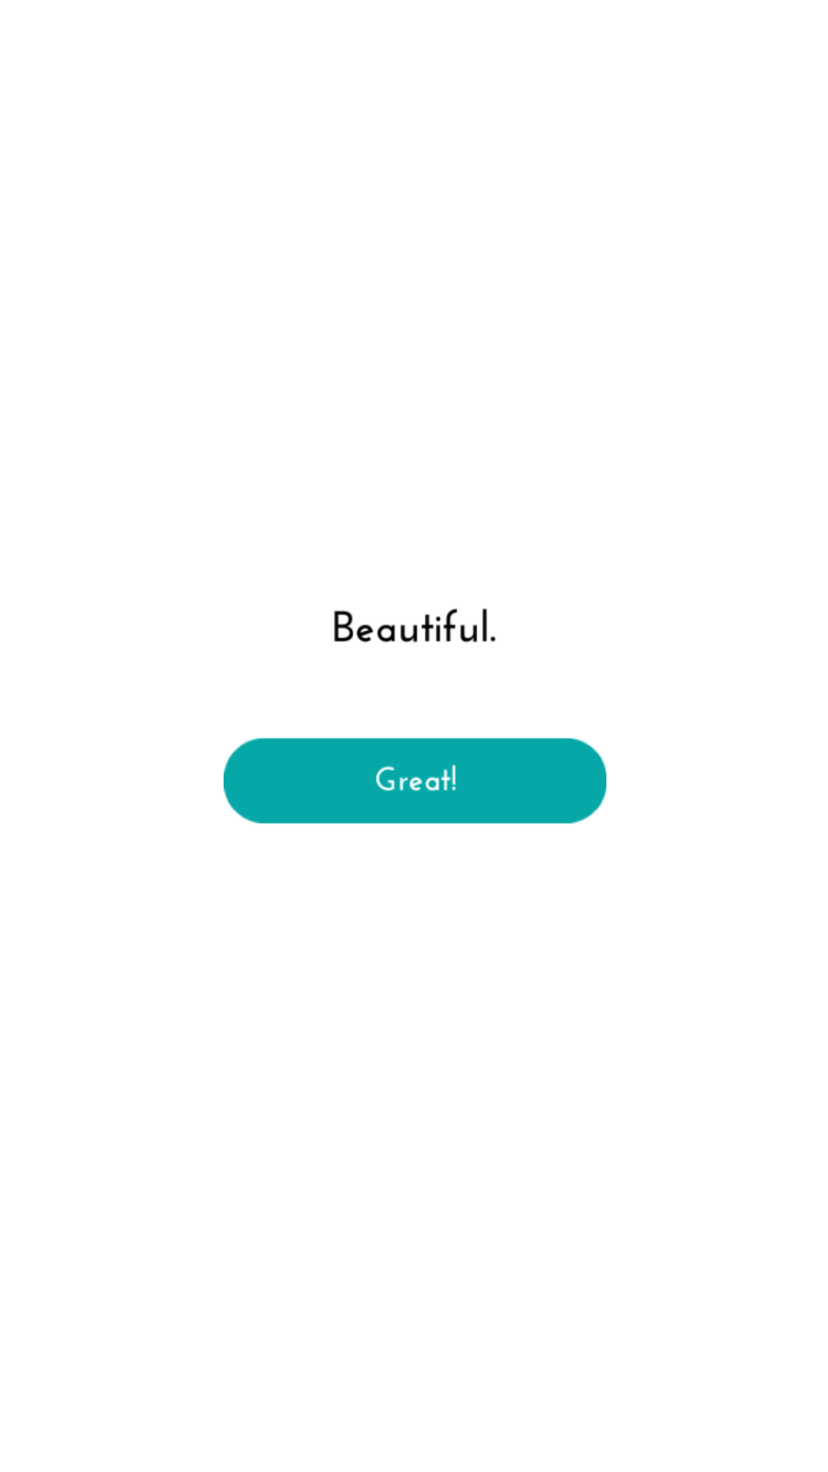
\includegraphics[width=.8\linewidth]{dots/2:2.png}
  \captionof{figure}{\\Positive reinforcement}
  \label{fig:2:2}
\end{minipage}
\end{figure}

As we start connecting the dots we can notice that the line at the bottom and top of the screen gets longer as we connect more, so we can deduce that this represent the length of the joined segments. If we connect the dots like in figure \ref{fig:1:7} the dots fall down and we get to start over at figure \ref{fig:1:6}. We only get to proceed if we manage to form a square with the lines as in figure \ref{fig:2:1}. This hints to us as users that it is better to form a square if possible than merely connecting the four dots, but we do not yet know why it is better.

After making a square with the four dots, we get some positive reinforcement, and we get to exclaim "Great!" by pressing the green button in figure \ref{fig:2:2}.

\begin{figure}
\centering
\captionsetup{format=multiline,font=footnotesize}
\begin{minipage}{.33333\textwidth}
  \centering
  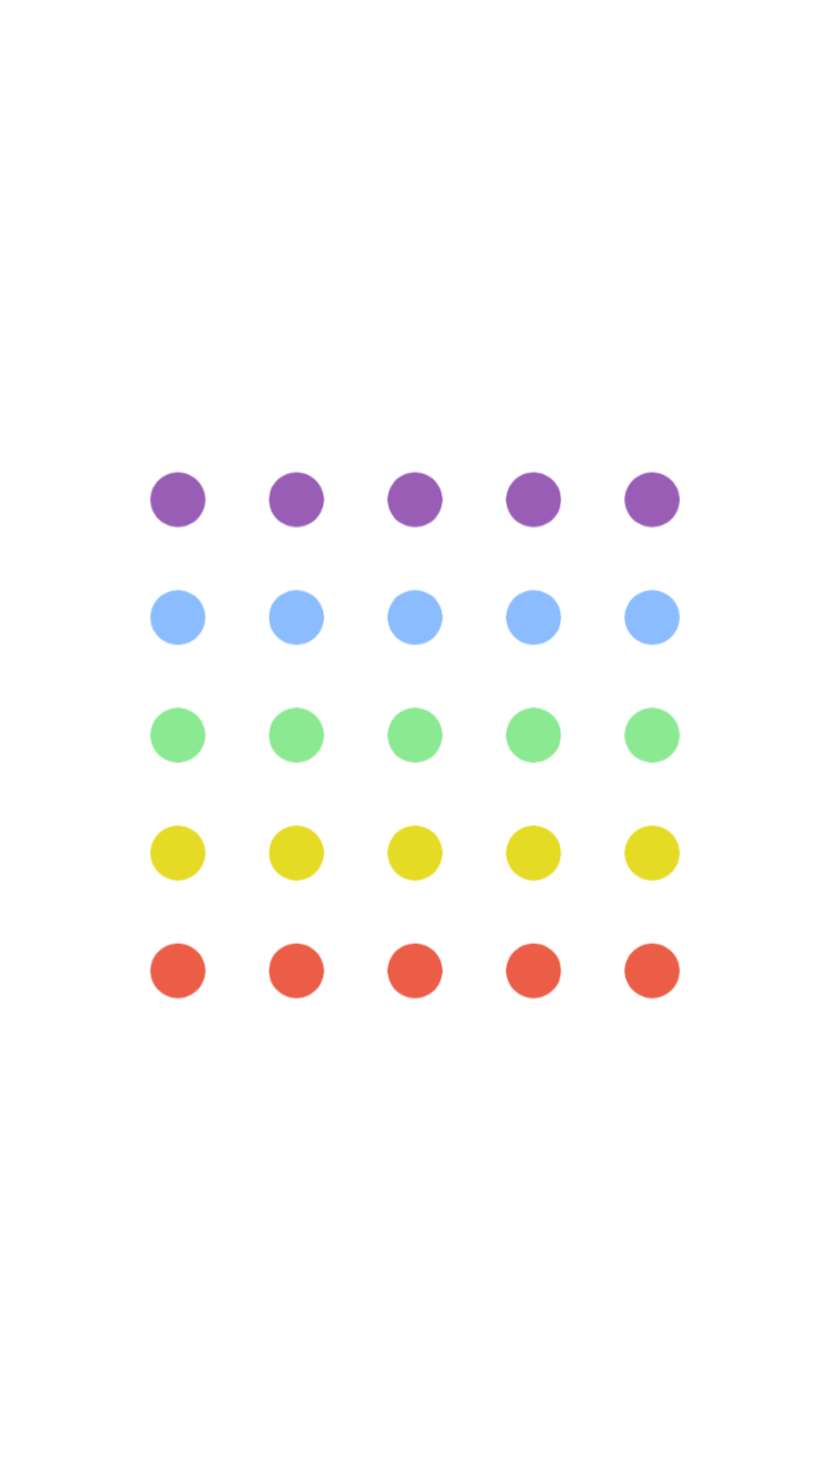
\includegraphics[width=.8\linewidth]{dots/2:3.png}
  \captionof{figure}{\\Lines with different colored dots}
  \label{fig:2:3}
\end{minipage}%
\begin{minipage}{.33333\textwidth}
  \centering
  
\includegraphics[width=.8\linewidth]{dots/2:4.png}
  \captionof{figure}{\\Connecting the lines}
  \label{fig:2:4}
\end{minipage}%
\begin{minipage}{.33333\textwidth}
  \centering
  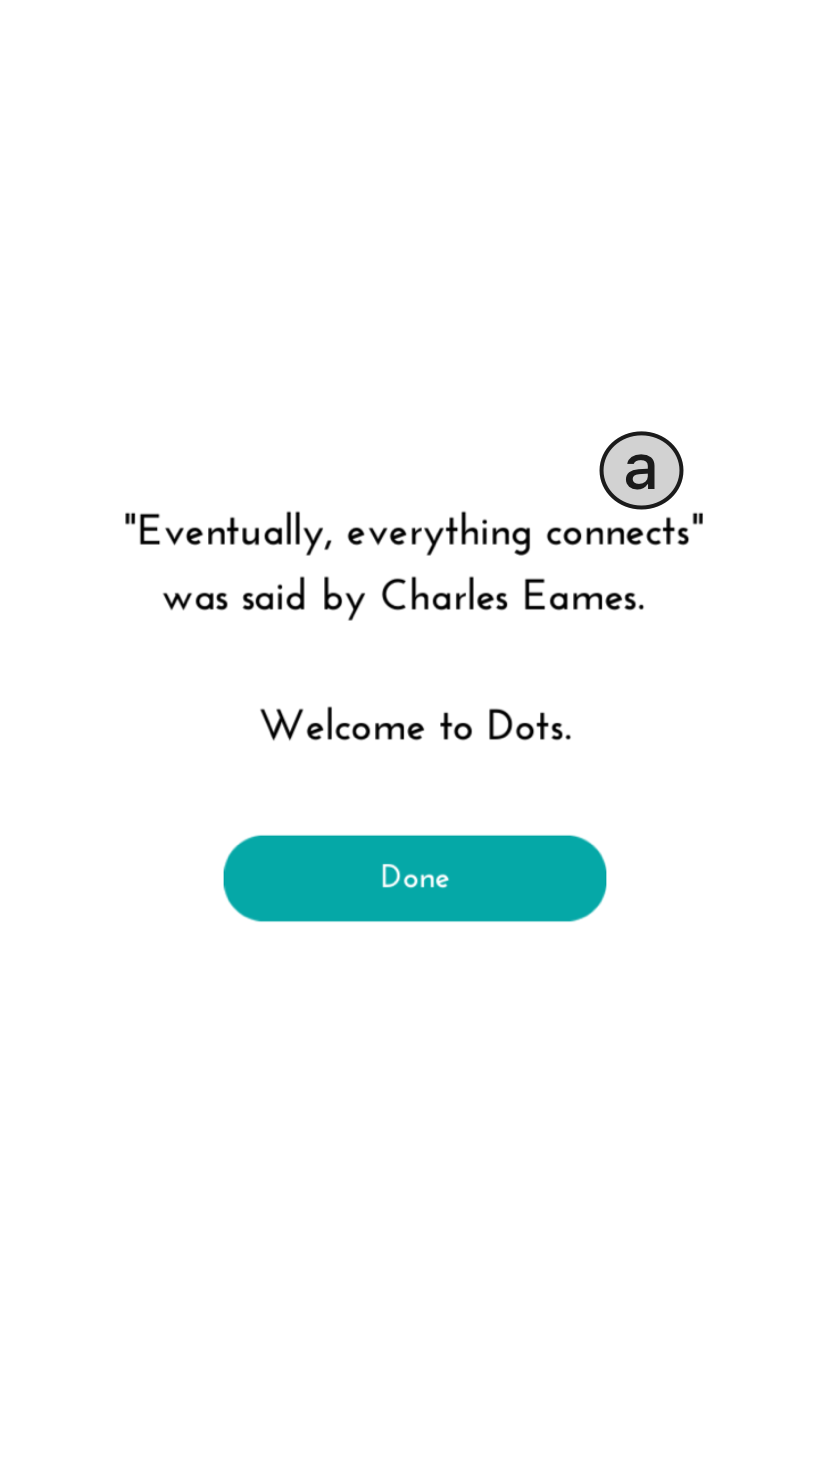
\includegraphics[width=\linewidth]{dots/2:5.png}
  \captionof{figure}{\\Final prompt of the interactive tutorial}
  \label{fig:2:5}
\end{minipage}
\end{figure}

After pressing "Great!" in figure \ref{fig:2:2} we're presented with an array of dots (Figure \ref{fig:2:3}). Unlike before, this time we're not prompted to do any specific task, but with our newly acquired experience and the order of the colored dots hints to us to connect them in lines, like in figure \ref{fig:2:4}. When there are no more dots to connect we get to proceed to figure \ref{fig:2:5}, and we get the same quote we were first presented with when we opened the app, but now we know that it was Charles Eames who said it. We proceed from here by pressing the only button with the label "Done".

\begin{figure}
\centering
\captionsetup{format=multiline,font=footnotesize}
\begin{minipage}{.33333\textwidth}
  \centering
  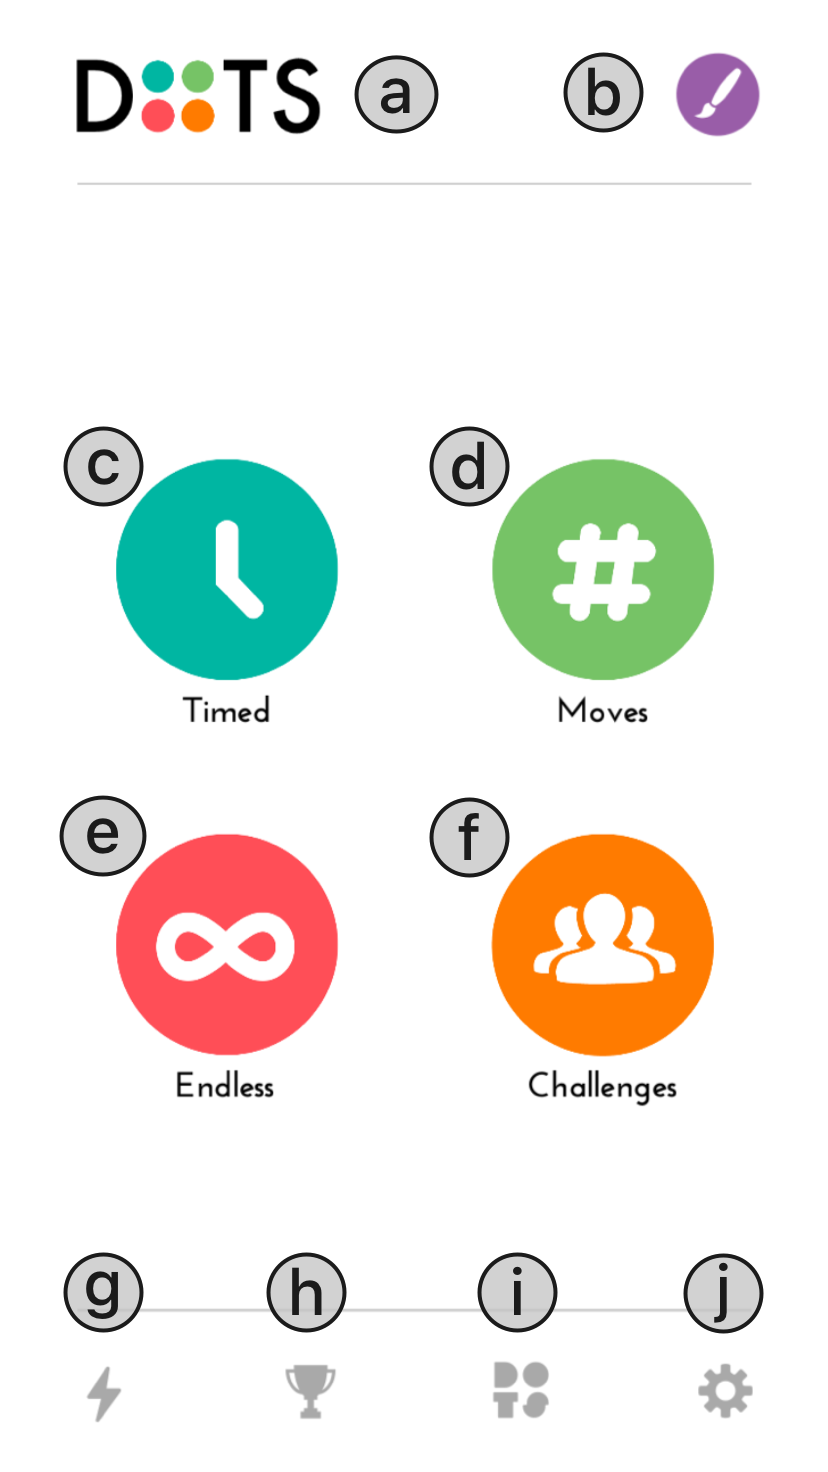
\includegraphics[width=.8\linewidth]{dots/2:6.png}
  \captionof{figure}{\\The main menu}
  \label{fig:2:6}
\end{minipage}%
\begin{minipage}{.33333\textwidth}
  \centering
  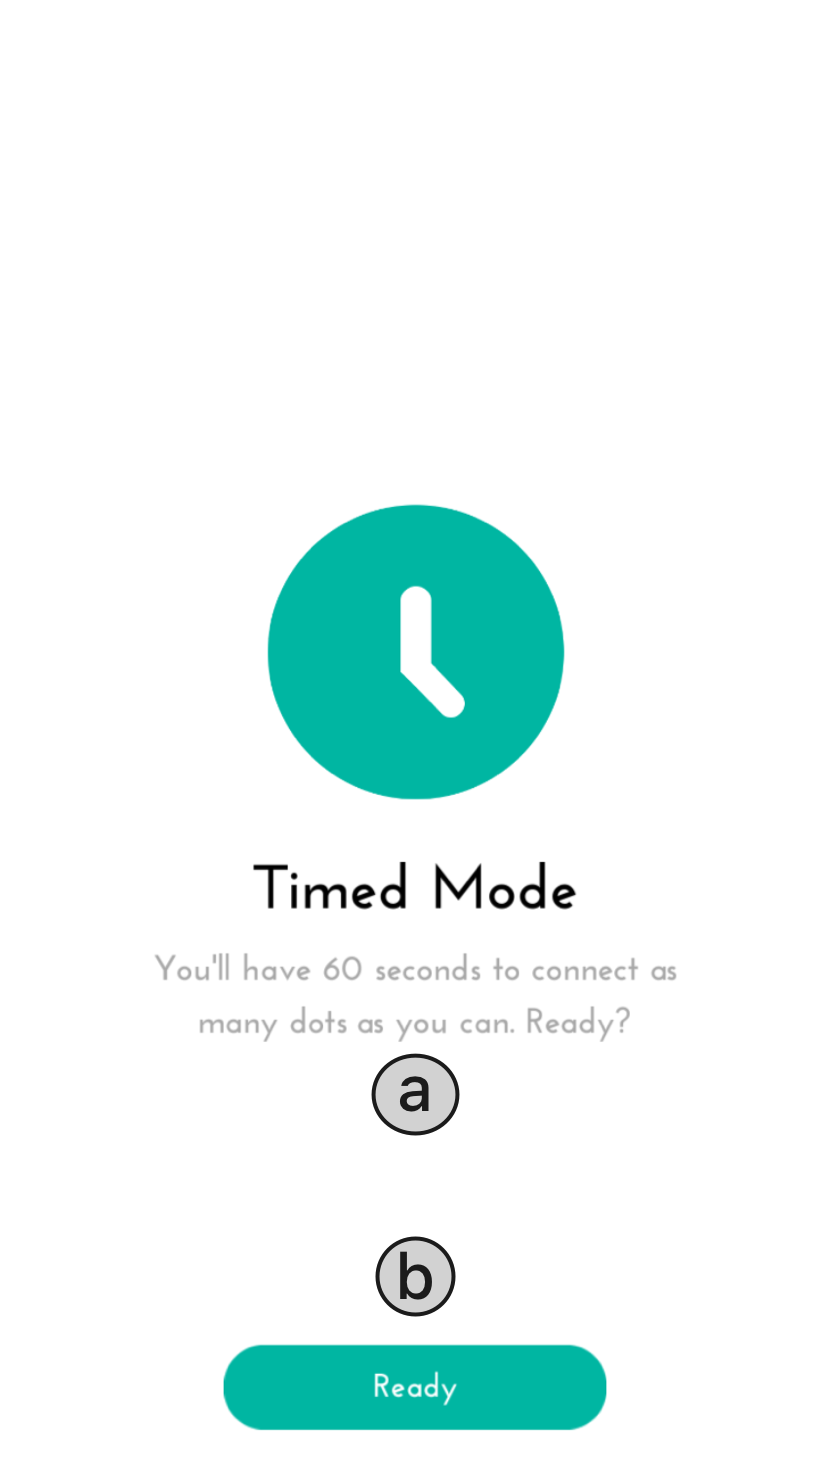
\includegraphics[width=.8\linewidth]{dots/2:7.png}
  \captionof{figure}{\\Timed mode description}
  \label{fig:2:7}
\end{minipage}%
\begin{minipage}{.33333\textwidth}
  \centering
  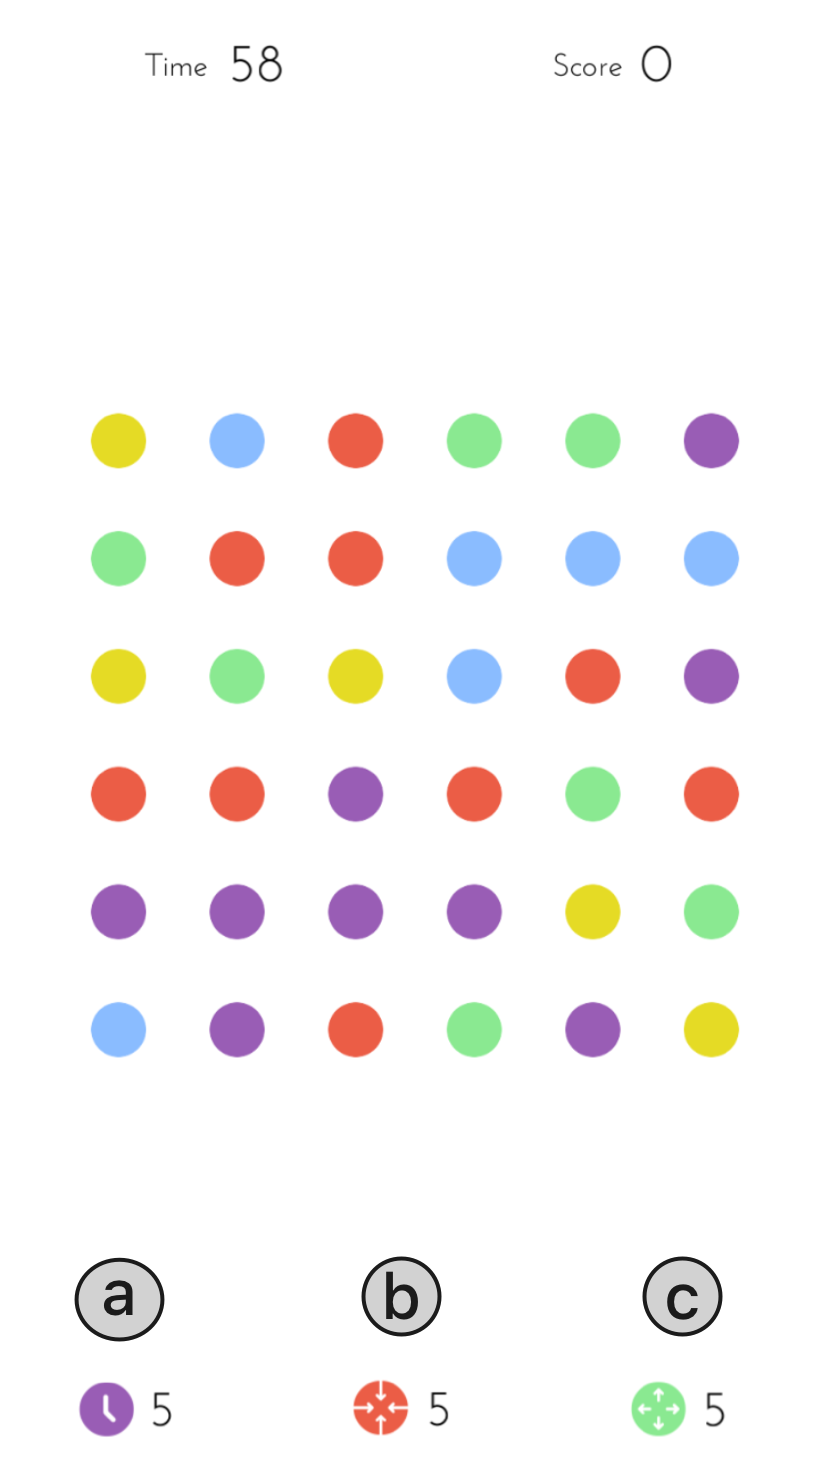
\includegraphics[width=\linewidth]{dots/3:1.png}
  \captionof{figure}{\\Game screen}
  \label{fig:3:1}
\end{minipage}
\end{figure}

Proceeding from figure \ref{fig:2:5} we're presented with the main menu of the application, and we're presented with seemingly 10 options. Nothing seems to happen when we press the logo of the app (a), (b) hints us that it takes us to some customization options of the app, (c-f) seem to be the main options of the app because of their large size and position in the center. (g-j) are the most vague possible options, with no labels and iconography that may be hard to figure out in the context of the app what they represent. Some possible options (b-f) are represented with round buttons -- (c-f) are labeled, while others (g-j) are represented with just icons.


%% The best practice evaluation will present 3 different applications and an evaluation of its interface and onboarding experience
\include{chapters/Best_practice_evalution}

%% The result chapter will contain the results from the expert interviews, any eventual framework remarks, user tests, personas and prototypes.
\chapter{Result}
% Carry out the research design that you described in the previous chapter.
% Describe how the research went and analyze the result.

\section{Literature study}
%
\section{Interviews}
%
\section{Best Practice Evaluation}
%
\section{Application review}
%
\section{User Testing}
%
\section{Personas}
%
\section{Prototypes}
%


%% The discussion chapter will discuss the results found of the study and its implications.
\chapter{Discussion}
\label{chap:discussion}

The following chapter will first discuss the major validity of the framework in regards to the results in \ref{chap:result}. Secondly, we discuss limitations and drawbacks of the individual results in chapter \ref{chap:result} and their implication on the thesis.

\section{Validity}

The result of the thesis managed to prove quantitatively that the test participants expected ease of use and usefulness was exceeded after the use of the prototype, assuming that the recorded samples are from a normal distribution. From the qualitative result of the usability test, we can conclude that the test participants enjoyed the use of the prototype. With these results in mind, we also have to consider that
\begin{enumerate*}[label=(\(\arabic*\))]
  \item \label{enum:original-app}The conceptual app design, as designed without the framework, could have produced the same or similar results,
  \item \label{enum:framework-aspects}not all aspects of the framework was applied to the prototype,
  \item \label{enum:app-aspects}not all functionality and aspects of the reviewed app has been covered by the framework, and finally
  \item \label{enum:experience}another designer, with the aid of the framework, could have produced a different onboarding solution
\end{enumerate*}

For the case of \ref{enum:original-app},  testing the conceptual app design was not possible since the scope of the design did not include essential onboarding functionality (e.g. the user login, the creation of a grocery list etc). Time constraints were the main contributing factor to \ref{enum:framework-aspects} and \ref{enum:app-aspects}, that not all aspects of the framework were applied to the design. The fact that the framework is general and at times have a high abstraction level is the main contributor to \ref{enum:experience}.

\section{Limitations \& Drawbacks}
\subsection{Personas}
The personas designed was made to be as representative of the survey results as possible. The accurateness of the personas is limited by the results of the survey and the design of the survey, which is discussed in Section \ref{sec:discussion/survey} below.

\subsection{Survey}
\label{sec:discussion/survey}
A few of the questions in the survey could have been better formulated/designed. For instance, the options to question number six "I usually shop in bulk" was a Likert scale of 1---7 which indicated how much they agree with the statement (1: I disagree completely, 7: I agree completely). The survey results for this question can be quite hard to analyze, and the options should have rather consisted of likert style items to indicate how often they go to a store to shop in bulk, similar to question five.

The impact of this on the personas is minor since we believe we managed to get create representative personas none the less.

\subsection{Framework Remarks}
Analyzing the mobileapp app and its design with the framework could have yielded different results by another person since the framework is general and some aspects can have a high level of abstraction. Not all framework remarks was implemented in the prototype due to time constraints, for example, the proposed added functionality to recipes.

\subsection{Usability test}

Below are some general ways to improve the usability tests conducted:

\begin{description}
  \item[Tasks] The number of tasks identified could have been larger, but even if we would have identified more tasks we would not be able to test them all due to time constraints.
  \item[Scenarios] The number of scenarios could have been reduced by "merging" similar scenarios into one.
  \item[Measurements] The audio during the user tests could have been recorded. Even though the test supervisor managed to document the most critical events and comments of the test participant audio recording would have helped when reviewing the results of the scenarios.
\end{description}

\section{Future work}

\begin{description}
  \item[Validation] The framework can be more thoroughly validated through further user tests and its application on different types of mobile applications. A better validation method and study could also be applied to the study.
  \item[Theoretical Background] More theoretical models and research can be included in the theoretical background to further strengthen it, especially the acceleration and assimilation part of it.
  \item[Platform] The framework could be expanded to include tablets, which would introduce further research to the framework.
\end{description}

% WRITE IN PRESENT TENSE

% In the discussion, you write mor interpretatively and colorfully about the results. Whereas you kept it concise in the conclusion, you write more in-depth about the subject in the discussion section.
% Evaluate the research: you may discuss your expectations of possible causes of and consequences of the results, possible limitations and suggestions for follow-up research.

% Start your discussion with the validity of your research. Then discuss the results and indicate whether they meet your expectations.
% In this section, you will give explanations for meeting or not meeting these expectations.
% Describe how your results fit with the framework that you have drawn in the first chapter (introduction, motivation, theoretical framework, and research questions/hypotheses).
%Show how the finding provide new or different insights into what was already known.

% Present the limitation of your research in a new paragraph within the discussion. Describe which observations you can make based on the research results.
% If there are some side notes that can be made to the research or you were hindered by certain limitations, these issues can explain of the results you obtained.
% Name these, but also explain how there factors can be improved in the future research.

%% --------------------------- CHECKLIST -------------------------------------
% - The validity of the research is demonstrated.
% - New insights are explained.
% - The limitations of the research are discussed.
% - It is indicated whether expectations were justified.
% - Possible causes and consequences of the results are discussed.
% - Suggestions for possible follow-up research are made.
% - Own interpretations have been included in the discussion.
% - There are no suggestions for follow-up research that are too vague.


%% The chapter Conclusion will conclude the study.
\chapter{Conclusion}
\label{chap:conclusion}
% PRESENT TENSE
% Should be between 200-400 words.

% Answer your research question. Reiterate the research question, but integrate an explanation of it into the rest of the sections discussion.

%% --------------------------- CHECKLIST -------------------------------------
% - The research questions have been answered.
% - The main question or problem statement has been answered.
% - The hypotheses have been confirmed or refused.
% - The right verb tense has been used.
% - No issues are interpreted.
% - No new information has been given.
% - No examples are used.
% - No extraneous information is provided.
% - No passages from the results have been cut and pasted.
% - The first person has not been used.




%%-----------------------------------------------------------------------------------------------------------------
%%----------------APPENDIX----------------------------------------------------------------------------------
%%-----------------------------------------------------------------------------------------------------------------

\clearpage

\addcontentsline{toc}{chapter}{\bibname}
\bibliographystyle{unsrt}

\bibliography{library}

\appendix

\end{document}
